\documentclass[11pt]{report}
\usepackage{multicol,lipsum,microtype}
\usepackage[table, xcdraw,dvipsnames]{xcolor}
\usepackage[backend=biber]{biblatex}
\addbibresource{bib/main.bib}
\usepackage{vub}
\usepackage{listings}
\usepackage{lstautogobble}  % Fix relative indenting
\usepackage{xargs}
\usepackage{float}
\usepackage{tikz}
\usepackage{bytefield}
\usepackage{pgf-umlsd}
\usepackage{pgfplots}
\pgfplotsset{compat=1.16}
\usepackage{caption}
\usepackage{subcaption}
\usepackage{acronym}
\usepackage{mathtools}
\usepackage{amssymb}
\usepackage{amsmath}
\usepackage{zi4}            % Nice font

\definecolor{bluekeywords}{rgb}{0.13, 0.13, 1}
\definecolor{greencomments}{rgb}{0, 0.5, 0}
\definecolor{redstrings}{rgb}{0.9, 0, 0}
\definecolor{graynumbers}{rgb}{0.5, 0.5, 0.5}

\usepackage[colorinlistoftodos,prependcaption,textsize=tiny]{todonotes}
\newcommandx{\unsure}[2][1=]{\todo[linecolor=red,backgroundcolor=red!25,bordercolor=red,#1]{#2}}
\newcommandx{\change}[2][1=]{\todo[linecolor=blue,backgroundcolor=blue!25,bordercolor=blue,#1]{#2}}
\newcommandx{\info}[2][1=]{\todo[linecolor=OliveGreen,backgroundcolor=OliveGreen!25,bordercolor=OliveGreen,#1]{#2}}
\newcommandx{\improvement}[2][1=]{\todo[linecolor=Plum,backgroundcolor=Plum!25,bordercolor=Plum,#1]{#2}}
\newcommandx{\thiswillnotshow}[2][1=]{\todo[disable,#1]{#2}}

% \usetikzlibrary{external}
% \tikzexternalize[prefix=tikz/]
% \usepackage[a4paper,landscape,hmargin={1cm,1cm}]{geometry}
\usepackage{tikz-timing}[2014/10/29]
\usetikztiminglibrary[rising arrows]{clockarrows}
\usetikzlibrary{fit}
\usetikzlibrary{calc}
\usetikzlibrary{quotes}
\usetikzlibrary{positioning}
\usetikzlibrary{arrows,automata}
\usetikzlibrary{backgrounds,calc,shadings,shapes.arrows,shapes.symbols,shadows}

\tikzstyle{bag} = [align=center]

\makeatletter
\pgfkeys{/pgf/.cd,
  parallelepiped offset x/.initial=2mm,
  parallelepiped offset y/.initial=2mm
}
\pgfdeclareshape{parallelepiped}
{
  \inheritsavedanchors[from=rectangle] % this is nearly a rectangle
  \inheritanchorborder[from=rectangle]
  \inheritanchor[from=rectangle]{north}
  \inheritanchor[from=rectangle]{north west}
  \inheritanchor[from=rectangle]{north east}
  \inheritanchor[from=rectangle]{center}
  \inheritanchor[from=rectangle]{west}
  \inheritanchor[from=rectangle]{east}
  \inheritanchor[from=rectangle]{mid}
  \inheritanchor[from=rectangle]{mid west}
  \inheritanchor[from=rectangle]{mid east}
  \inheritanchor[from=rectangle]{base}
  \inheritanchor[from=rectangle]{base west}
  \inheritanchor[from=rectangle]{base east}
  \inheritanchor[from=rectangle]{south}
  \inheritanchor[from=rectangle]{south west}
  \inheritanchor[from=rectangle]{south east}
  \backgroundpath{
    % store lower right in xa/ya and upper right in xb/yb
    \southwest \pgf@xa=\pgf@x \pgf@ya=\pgf@y
    \northeast \pgf@xb=\pgf@x \pgf@yb=\pgf@y
    \pgfmathsetlength\pgfutil@tempdima{\pgfkeysvalueof{/pgf/parallelepiped
      offset x}}
    \pgfmathsetlength\pgfutil@tempdimb{\pgfkeysvalueof{/pgf/parallelepiped
      offset y}}
    \def\ppd@offset{\pgfpoint{\pgfutil@tempdima}{\pgfutil@tempdimb}}
    \pgfpathmoveto{\pgfqpoint{\pgf@xa}{\pgf@ya}}
    \pgfpathlineto{\pgfqpoint{\pgf@xb}{\pgf@ya}}
    \pgfpathlineto{\pgfqpoint{\pgf@xb}{\pgf@yb}}
    \pgfpathlineto{\pgfqpoint{\pgf@xa}{\pgf@yb}}
    \pgfpathclose
    \pgfpathmoveto{\pgfqpoint{\pgf@xb}{\pgf@ya}}
    \pgfpathlineto{\pgfpointadd{\pgfpoint{\pgf@xb}{\pgf@ya}}{\ppd@offset}}
    \pgfpathlineto{\pgfpointadd{\pgfpoint{\pgf@xb}{\pgf@yb}}{\ppd@offset}}
    \pgfpathlineto{\pgfpointadd{\pgfpoint{\pgf@xa}{\pgf@yb}}{\ppd@offset}}
    \pgfpathlineto{\pgfqpoint{\pgf@xa}{\pgf@yb}}
    \pgfpathmoveto{\pgfqpoint{\pgf@xb}{\pgf@yb}}
    \pgfpathlineto{\pgfpointadd{\pgfpoint{\pgf@xb}{\pgf@yb}}{\ppd@offset}}
  }
}
\makeatother

\definecolor{listing-background}{HTML}{F7F7F7}
\definecolor{listing-rule}{HTML}{B3B2B3}
\definecolor{listing-numbers}{HTML}{B3B2B3}
\definecolor{listing-text-color}{HTML}{000000}
\definecolor{listing-keyword}{HTML}{435489}
\definecolor{listing-keyword-2}{HTML}{1284CA} % additional keywords
\definecolor{listing-keyword-3}{HTML}{9137CB} % additional keywords
\definecolor{listing-identifier}{HTML}{435489}
\definecolor{listing-string}{HTML}{00999A}
\definecolor{listing-comment}{HTML}{8E8E8E}

\lstset{
  language         = C++,
  numbers          = left,
  xleftmargin      = 2.7em,
  framexleftmargin = 2.5em,
  backgroundcolor  = \color{listing-background},
  basicstyle       = \color{listing-text-color}\linespread{1.0}\small\ttfamily{},
  breaklines       = true,
  frame            = single,
  framesep         = 0.19em,
  rulecolor        = \color{listing-rule},
  frameround       = ffff,
  tabsize          = 4,
  numberstyle      = \color{listing-numbers},
  aboveskip        = 1.0em,
  belowskip        = 0.1em,
  abovecaptionskip = 0em,
  belowcaptionskip = 1.0em,
  keywordstyle     = {\color{listing-keyword}\bfseries},
  keywordstyle     = {[2]\color{listing-keyword-2}\bfseries},
  keywordstyle     = {[3]\color{listing-keyword-3}\bfseries\itshape},
  sensitive        = true,
  identifierstyle  = \color{listing-identifier},
  commentstyle     = \color{listing-comment},
  stringstyle      = \color{listing-string},
  showstringspaces = false,
  escapeinside     = {/*@}{@*/}, % Allow LaTeX inside these special comments
  literate         =
  {á}{{\'a}}1 {é}{{\'e}}1 {í}{{\'i}}1 {ó}{{\'o}}1 {ú}{{\'u}}1
  {Á}{{\'A}}1 {É}{{\'E}}1 {Í}{{\'I}}1 {Ó}{{\'O}}1 {Ú}{{\'U}}1
  {à}{{\`a}}1 {è}{{\'e}}1 {ì}{{\`i}}1 {ò}{{\`o}}1 {ù}{{\`u}}1
  {À}{{\`A}}1 {È}{{\'E}}1 {Ì}{{\`I}}1 {Ò}{{\`O}}1 {Ù}{{\`U}}1
  {ä}{{\"a}}1 {ë}{{\"e}}1 {ï}{{\"i}}1 {ö}{{\"o}}1 {ü}{{\"u}}1
  {Ä}{{\"A}}1 {Ë}{{\"E}}1 {Ï}{{\"I}}1 {Ö}{{\"O}}1 {Ü}{{\"U}}1
  {â}{{\^a}}1 {ê}{{\^e}}1 {î}{{\^i}}1 {ô}{{\^o}}1 {û}{{\^u}}1
  {Â}{{\^A}}1 {Ê}{{\^E}}1 {Î}{{\^I}}1 {Ô}{{\^O}}1 {Û}{{\^U}}1
  {œ}{{\oe}}1 {Œ}{{\OE}}1 {æ}{{\ae}}1 {Æ}{{\AE}}1 {ß}{{\ss}}1
  {ç}{{\c c}}1 {Ç}{{\c C}}1 {ø}{{\o}}1 {å}{{\r a}}1 {Å}{{\r A}}1
  {€}{{\EUR}}1 {£}{{\pounds}}1 {«}{{\guillemotleft}}1
  {»}{{\guillemotright}}1 {ñ}{{\~n}}1 {Ñ}{{\~N}}1 {¿}{{?`}}1
  {…}{{\ldots}}1 {≥}{{>=}}1 {≤}{{<=}}1 {„}{{\glqq}}1 {“}{{\grqq}}1
  {”}{{''}}1
}
\lstdefinelanguage{none}{
  identifierstyle=,
  commentstyle=,
  stringstyle=,
  keywordstyle=,
}

\def\lav{lavander!90}
\def\oran{orange!30}

\tikzstyle{motes}=[draw,circle,bottom color= gray,
                  top color= white,minimum width=10pt]
\tikzstyle{gateways}=[draw,circle, left color= orange,minimum width=20pt]

\tikzset{l3 switch/.style={
    minimum width=0.75cm,
    minimum height=0.75cm,
    parallelepiped,fill=switch, draw=white,
    parallelepiped offset x=1.75mm,
    parallelepiped offset y=1.25mm,
    path picture={
      \node[fill=white,
        circle,
        minimum size=6pt,
        inner sep=0pt,
        append after command={
          \pgfextra{
            \foreach \angle in {0,45,...,360}
            \draw[-latex,fill=white] (\tikzlastnode.\angle)--++(\angle:2.25mm);
          }
        }
      ] 
       at ([xshift=-0.75mm,yshift=-0.5mm]path picture bounding box.center){};
    }
  },
  ports/.style={
    line width=0.3pt,
    top color=gray!20,
    bottom color=gray!80
  },
  rack switch/.style={
    minimum width=1.25cm,
    minimum height=0.25cm,
    parallelepiped,fill=white, draw,
    parallelepiped offset x=2mm,
    parallelepiped offset y=1.25mm,
    xscale=-1,
    path picture={
      \draw[top color=gray!5,bottom color=gray!40]
      (path picture bounding box.south west) rectangle 
      (path picture bounding box.north east);
      \coordinate (A-west) at ([xshift=-0.2cm]path picture bounding box.west);
      \coordinate (A-center) at ($(path picture bounding box.center)!0!(path
        picture bounding box.south)$);
      \foreach \x in {0.275,0.525,0.775}{
        \draw[ports]([yshift=-0.05cm]$(A-west)!\x!(A-center)$)
          rectangle +(0.1,0.05);
        \draw[ports]([yshift=-0.125cm]$(A-west)!\x!(A-center)$)
          rectangle +(0.1,0.05);
       } 
      \coordinate (A-east) at (path picture bounding box.east);
      \foreach \x in {0.085,0.21,0.335,0.455,0.635,0.755,0.875,1}{
        \draw[ports]([yshift=-0.1125cm]$(A-east)!\x!(A-center)$)
          rectangle +(0.05,0.1);       
      }
    }
  },
  server/.style={
    fill=white, draw,
    minimum width=0.35cm,
    minimum height=0.75cm,
    parallelepiped,
    parallelepiped offset x=3mm,
    parallelepiped offset y=2mm,
    xscale=-1,
    path picture={
      \draw[top color=gray!5,bottom color=gray!40]
      (path picture bounding box.south west) rectangle 
      (path picture bounding box.north east);
      \coordinate (A-center) at ($(path picture bounding box.center)!0!(path
        picture bounding box.south)$);
      \coordinate (A-west) at ([xshift=-0.575cm]path picture bounding box.west);
      \draw[ports]([yshift=0.1cm]$(A-west)!0!(A-center)$)
        rectangle +(0.2,0.065);
      \draw[ports]([yshift=0.01cm]$(A-west)!0.085!(A-center)$)
        rectangle +(0.15,0.05);
      \fill[black]([yshift=-0.35cm]$(A-west)!-0.1!(A-center)$)
        rectangle +(0.235,0.0175);
      \fill[black]([yshift=-0.385cm]$(A-west)!-0.1!(A-center)$)
        rectangle +(0.235,0.0175);
      \fill[black]([yshift=-0.42cm]$(A-west)!-0.1!(A-center)$)
        rectangle +(0.235,0.0175);
    }  
  },
}

\newcommand{\messdash}[4][0]{
  \stepcounter{seqlevel}
  \path
  (#2)+(0,-\theseqlevel*\unitfactor-0.7*\unitfactor) node (mess from) {};
  \addtocounter{seqlevel}{#1}
  \path
  (#4)+(0,-\theseqlevel*\unitfactor-0.7*\unitfactor) node (mess to) {};
  \draw[->,>=angle 60, dashed] (mess from) -- (mess to) node[midway, above]
  {#3};

  \node (#3 from) at (mess from) {};
  \node (#3 to) at (mess to) {};
}


\title{Master Thesis}
\subtitle{Toward Energy Efficient LoRa Multihop networks}
\author{Perale Thomas}
\faculty{Science and Bio-Engineering Sciences}
\promotors{Promotors: Prof. Dr. Ir. Kris Steenhaut, Prof. Dr. Eliza
Gonzalez Boix\newline Supervisor: Roald Van Glabbeek}
\pretitle{}

\def\triangleH{27.7mm}

\begin{document}
\maketitle

\pagenumbering{roman}

\section*{Abstract}

\newpage

\section*{Acknowledgement}

\newpage

\tableofcontents

\newpage

\listoffigures

\newpage

\section*{List of acronyms}

\begin{acronym}[MPC]
\acro{BW}{Bandwidth}
\acro{CAD}{Channel Activity Detection}
\acro{CCA}{Clear Channel Assessment}
\acro{CSS}{Chirp Spread Spectrum}
\acro{CSMA}{Carrier-Sense Multiple Access}
\acro{CR}{Coding Rate}
\acro{CRC}{Cyclic Redundancy Check}
\acro{FEC}{Forward Error Correction}
\acro{GW}{Gateway}
\acro{ISM}{Industrial, Scientific and Medical Band}
\acro{IT}{Information Technology}
\acro{IoT}{Internet of Things}
\acro{IIoT}{Industrial Internet of Things}
\acro{LLN}{Low Power and Lossy Networks}
\acro{LPWAN}{Low-power wide-area network}
\acro{PHY}{Physical layer}
\acro{SF}{Spreading Factor}
\acro{TSCH}{Time Slotted Channel Hopping}
\end{acronym}



\newpage

\pagenumbering{arabic}

\section{Introduction}

With each year new companies jumping into the \emph{IoT} sector and all the major \emph{IT actors} investing and developing products\footnote{https://www.fortunebusinessinsights.com/industry-reports/internet-of-things-iot-market-100307}, as well as telecoms building new infrastructure. The \emph{Internet of Things} has undoubtedly been a subject of hype during the last decade while still maintaining a consistent growth until now. 
Business analysts agree that we should expect to reach at least 40 billion installed \emph{IoT} devices by 2027\footnote{https://www.businessinsider.com/internet-of-things-report}. The \emph{Internet of Things} is used to describe inter-connected devices gathering data without the need of human interaction.
We are, as consumer, already familiar with the traditional \emph{IoT} products we use in our households that allow to connect our light bulbs, our fridge and washing machine, ...
Meanwhile we have less knowledge of the industrial usage of \emph{IoT}, also known as \emph{IIoT}. \emph{IIoT} is one of the fastest growing domain of the market. More and more industries are adopting \emph{IoT}  to consolidate their productions with \emph{real-time monitoring}, predictive maintenance on their assets and products, connecting their supply chains, all of this enabled with the help of network of sensors.
This is applicable in a wide spectrum of domains like \emph{smart farming}, \emph{smart cars}, \emph{smart cities}, \emph{energy managements}, ...

\paragraph{}

The common aspect of all of these applications are that they can communicate wirelessly.
A multitude of telecommunication technologies are used or were created to suit this solution and can be categorized by three different characteristics

\begin{itemize}
    \item Long or Short \emph{range}
    \item High or low \emph{data-rate}
    \item Low or high \emph{power usage} 
\end{itemize}

From these characteristics you can only chose two according to the physical law % TODO Explanation needed
The following graphics\ref{fig:commrangegraph} show a classification of the existing wireless communication used in the \emph{IoT} and mix the three main categories.

\begin{itemize}
    \item \emph{Short-Range wireless communication}
    \item \emph{Cellular communication}
    \item \emph{LPWAN communication} Long range, low power and low data-rate
\end{itemize}

\begin{figure}[H] % TODO More info on axis
\centering
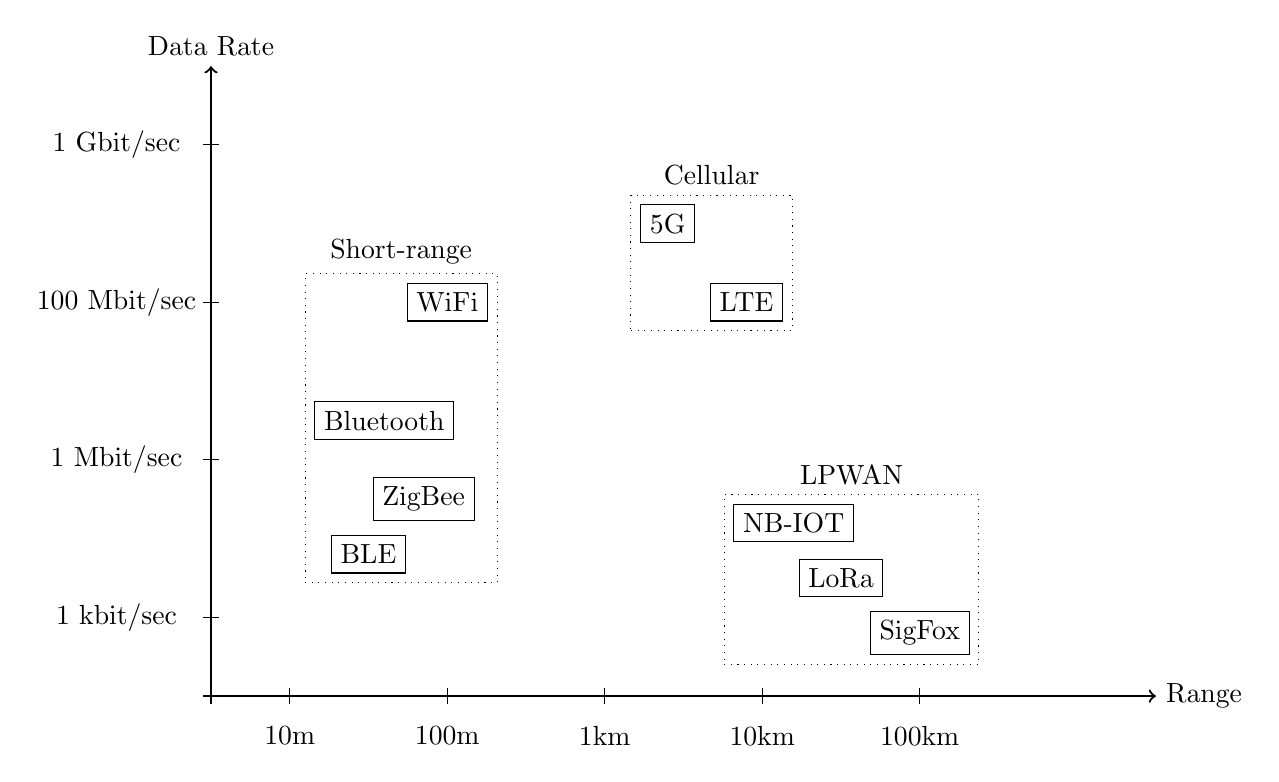
\begin{tikzpicture}
    \draw[->,thick] (-0.1,0)--(12,0) node[right]{Range};
    \draw[->,thick] (0,-0.1)--(0,8) node[above]{Data Rate};
    \node[] at (1, -0.5) {10m};
    \draw[] (1,-0.1)--(1,0.1);
    \node[] at (3, -0.5) {100m};
    \draw[] (3,-0.1)--(3,0.1);
    \node[] at (5, -0.5) {1km};
    \draw[] (5,-0.1)--(5,0.1);
    \node[] at (7, -0.5) {10km};
    \draw[] (7,-0.1)--(7,0.1);
    \node[] at (9, -0.5) {100km};
    \draw[] (9,-0.1)--(9,0.1);

    \node[] at (-1.2, 1) {1 kbit/sec};
    \draw[] (-0.1,1)--(0.1,1);
    \node[] at (-1.2, 3) {1 Mbit/sec};
    \draw[] (-0.1,3)--(0.1,3);
    \node[] at (-1.2, 5) {100 Mbit/sec};
    \draw[] (-0.1,5)--(0.1,5);
    \node[] at (-1.2, 7) {1 Gbit/sec};
    \draw[] (-0.1,7)--(0.1,7);
    
    \node[draw] at (8,1.5) (lora) {LoRa};
    \node[draw] at (9.0,0.8) (sigfox) {SigFox};
    \node[draw] at (7.4,2.2) (nb) {NB-IOT};
    \node[draw,dotted,fit=(lora) (sigfox) (nb), label=above:{LPWAN}] {};

    
    \node[draw] at (2.2,3.5) (bluetooth) {Bluetooth};
    \node[draw] at (2.7,2.5) (zigbee) {ZigBee};
    \node[draw] at (2.0,1.8) (ble) {BLE};
    \node[draw] at (3,5) (wifi) {WiFi};
    \node[draw,dotted,fit=(bluetooth) (zigbee) (ble) (wifi), label=above:{Short-range}] {};

    \node[draw] at (6.8,5) (lte) {LTE};
    \node[draw] at (5.8,6) (5g) {5G};
    \node[draw,dotted,fit=(lte) (5g), label=above:{Cellular}] {};
\end{tikzpicture}
\caption{Comparison of the existing IoT wireless technologies by range and data rate}
\label{fig:commrangegraph}
\end{figure}


This work focus only on \emph{LoRa}, a proprietary chirp spread spectrum modulation technique owned by \emph{Semtech} operating in the sub-GHz unlicensed \emph{ISM} band, that will be explained in more details in section \ref{section:lora}.
The main characteristics of \emph{LoRa} is that it trade throughput for range and low power transmission that as already achieved a record distance of 700km with direct line of sight between the receiver and the transmitter\footnote{https://www.thethingsnetwork.org/article/ground-breaking-world-record-lorawan-packet-received-at-702-km-436-miles-distance}. However this case is not a real world example, we should expect a typical range in urban areas of around \emph{~2-5km} and \emph{15km} in suburban areas\cite{8030482}. Fine tuning the \emph{PHY} settings of the protocol also allow to trade communication distance over throughput and a longer band usage which decrease the number of concurrent motes that can communicate over the band\cite{10.1145/2988287.2989163}.

\emph{LoRa} is often used in conjunction with the \emph{LoRaWAN} a point-to-multipoint protocols. \emph{LoRaWAN} is a ALOHA based\cite{loraalliance:lorawanspecification} network using a star-of-stars topology composed of
wirelessly interconnected \emph{motes} sending data to \emph{gateways} which relay messages to central servers over a Cellular or Ethernet connection as we can see in Figure \ref{fig:startopology}.

\begin{figure}[H]
\begin{subfigure}[b]{.5\textwidth}
    \centering
    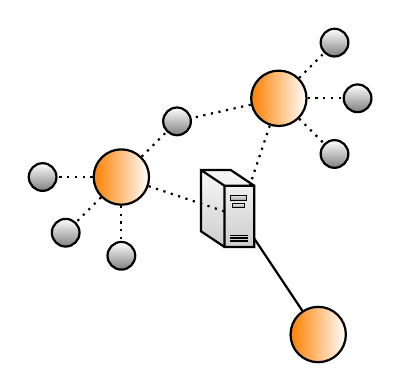
\begin{tikzpicture}[auto, thick]
      % Place super peers and connect them
      \foreach \place/\name in {{(0,-1)/a}, {(2,0)/b}, {(2.5, -3)/c}}
        \node[gateways] (\name) at \place {};
      \node[server] (d) at (1.5,-1.5) {};
      %
      \foreach \source/\dest in {a/d, b/d}
        \path[dotted] (\source) edge (\dest);
      \path (c) edge (d); % Non dotted
      %
      % Place normal peers
      \foreach \pos/\i in {above right of/1, right of/2, below right of/3}
        \node[motes, \pos =b ] (b\i) {};
      \foreach \speer/\peer in {b/b1,b/b2,b/b3}
        \path[dotted] (\speer) edge (\peer);
      %
      \foreach \pos/\i in {below left of/1, below of/2, left of/3, above right of/4}
        \node[motes, \pos =a ] (a\i) {};
      \foreach \speer/\peer in {a/a1,a/a2,a/a3,a/a4}
        \path[dotted] (\speer) edge (\peer);
      %
      \path[dotted] (b) edge (a4);
    \end{tikzpicture}
    \caption{Star topology}
    \label{fig:startopology}
\end{subfigure}
\hfill
\begin{subfigure}[b]{.5\textwidth}
    \centering
    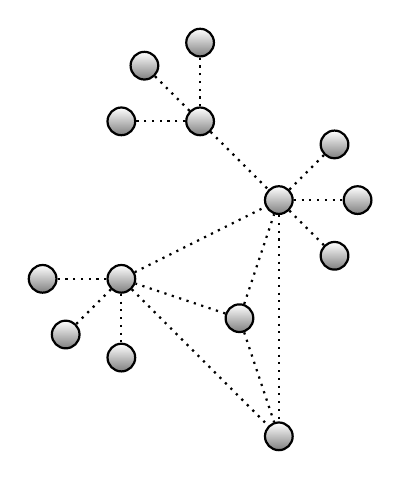
\begin{tikzpicture}[auto, thick]
      % Place super peers and connect them
      \foreach \place/\name in {{(0,-1)/a}, {(2,0)/b}, {(2, -3)/c}, {(1,1)/d}, {(1.5, -1.5)/f}}
        \node[motes] (\name) at \place {};
      \foreach \source/\dest in {a/b, a/c, b/c, d/b, f/a, f/b, f/c}
        \path[dotted] (\source) edge (\dest);
      %
      % Place normal peers
      \foreach \pos/\i in {above right of/1, right of/2, below right of/3}
        \node[motes, \pos =b ] (b\i) {};
      \foreach \speer/\peer in {b/b1,b/b2,b/b3}
        \path[dotted] (\speer) edge (\peer);
      %
      \foreach \pos/\i in {above left of/1, left of/2, above of/3}
        \node[motes, \pos =d ] (d\i) {};
      \foreach \speer/\peer in {d/d1,d/d2,d/d3}
        \path[dotted] (\speer) edge (\peer);
      %
      \foreach \pos/\i in {below left of/1, below of/2, left of/3}
        \node[motes, \pos =a ] (a\i) {};
      \foreach \speer/\peer in {a/a1,a/a2,a/a3}
        \path[dotted] (\speer) edge (\peer);
    \end{tikzpicture}
    \caption{Mesh Network Topology}
    \label{fig:meshtopology}
\end{subfigure}
\caption{Different LoRa Network Topologies}
\label{fig:topologies}
\end{figure}




The issue we have is \emph{LoRaWAN} does not scale\cite{10.1145/2988287.2989163}, especially in an urban environment where a lot of motes could overlap. \emph{LoRaWAN} is \emph{ALOHA} based and\emph{CSMA} is not possible because \emph{Channel Activity Detection} only detect the preamble of a communication. This mean a lot of collision can occur during a transmission attempt with a gateway. The \emph{LoRaWAN} protocol state that on collision occur the transmission has to be re-done which lead to a bigger energy consumption as well as occupying the channel even more.
Link quality may also vary some motes far away from the gateway may have issue with doing a correct transmission. Environmental factor like temperature, humidity\cite{evaluation_of_the_reliability_of_lora}, have a lot of influence in the link quality.

Also gateways may not be available everywhere, some use cases may not allow the the installation of gateways, which would imply a power and internet connection, that's the case for pipelines and tunnel, % cite here TODO
where we would prefer to only run devices on batteries.

\begin{figure}[H]
    \centering
    \def\angle{0}
    \def\radius{3}
    \begin{tikzpicture}[nodes = {font=\sffamily}]
      \foreach \color in {
            yellow,
            red,
            yellow,
            white,
            red,
            yellow,
            white,
            yellow,
            white,
            white,
            red,
            red,
        } {
        \ifx\color\empty\else
            \draw[fill={\color!50},draw={\color}] (0,0) -- (\angle:\radius)
              arc (\angle:\angle+30:\radius) -- cycle;
            \pgfmathparse{\angle+30}
            \xdef\angle{\pgfmathresult}
        \fi
        };
        \xdef\radius{2.5}
        \foreach \color in {
            yellow,
            red,
            yellow,
            yellow,
            red,
            white,
            yellow,
            red,
            white,
            white,
            white,
            white,
        } {
        \ifx\color\empty\else
            \draw[fill={\color!50},draw={\color}] (0,0) -- (\angle:\radius)
              arc (\angle:\angle+30:\radius) -- cycle;
            \pgfmathparse{\angle+30}
            \xdef\angle{\pgfmathresult}
        \fi
        };
        \xdef\radius{2}
        \foreach \color in {
            yellow,
            red,
            green,
            red,
            yellow,
            white,
            yellow,
            white,
            white,
            white,
            white,
            white,
        } {
        \ifx\color\empty\else
            \draw[fill={\color!50},draw={\color}] (0,0) -- (\angle:\radius)
              arc (\angle:\angle+30:\radius) -- cycle;
            \pgfmathparse{\angle+30}
            \xdef\angle{\pgfmathresult}
        \fi
        };
        \xdef\radius{1.5}
        \foreach \color in {
            yellow,
            red,
            yellow,
            yellow,
            yellow,
            green,
            yellow,
            white,
            red,
            white,
            white,
            white,
        } {
        \ifx\color\empty\else
            \draw[fill={\color!50},draw={\color}] (0,0) -- (\angle:\radius)
              arc (\angle:\angle+30:\radius) -- cycle;
            \pgfmathparse{\angle+30}
            \xdef\angle{\pgfmathresult}
        \fi
        };
        \xdef\radius{1}
        \foreach \color in {
            green,
            green,
            green,
            yellow,
            yellow,
            yellow,
            white,
            white,
            yellow,
            red,
            yellow,
            red,
        } {
        \ifx\color\empty\else
            \draw[fill={\color!50},draw={\color}] (0,0) -- (\angle:\radius)
              arc (\angle:\angle+30:\radius) -- cycle;
            \pgfmathparse{\angle+30}
            \xdef\angle{\pgfmathresult}
        \fi
        };
        \xdef\radius{0.5}
        \foreach \color in {
            green,
            green,
            yellow,
            yellow,
            green,
            green,
            yellow,
            red,
            yellow,
            green,
            green,
            green,
        } {
        \ifx\color\empty\else
            \draw[fill={\color!50},draw={\color}] (0,0) -- (\angle:\radius)
              arc (\angle:\angle+30:\radius) -- cycle;
            \pgfmathparse{\angle+30}
            \xdef\angle{\pgfmathresult}
        \fi
        };
    \end{tikzpicture}
\caption{Typical gateway coverage\cite{lorajambalaya}}
\label{fig:coverage}

\begin{tabular}{r@{: }l r@{: }l}

\begin{tikzpicture}\draw[fill=green,line width=1pt]  circle(1ex);\end{tikzpicture} & Good\ Connection & 
\begin{tikzpicture}\draw[fill=yellow,line width=1pt]  circle(1ex);\end{tikzpicture} & Intermediate\ Connection\\

\begin{tikzpicture}\draw[fill=red,line width=1pt]  circle(1ex);\end{tikzpicture} & Bad\ Connection & 
\begin{tikzpicture}\draw[fill=white,line width=1pt]  circle(1ex);\end{tikzpicture} & No\ Connection 
\end{tabular}
\end{figure}




% \begin{tikzpicture}
%     \node[draw] (Application) [abstract, rectangle]{\textbf{Application Layer}};
%     \node[draw] (MAC) [abstract, rectangle, below=0.2cm of Application, text justified]{\textbf{Media Access Control (MAC) Layer}};
%     \node[draw] (Phy) [abstract, rectangle, below=0.2cm of MAC, text justified]{\textbf{Physical (PHY) Layer}};
%     \node[draw] (Rf) [abstract, rectangle, below=0.2cm of Phy, text justified]{\textbf{Radio Frequency (RF) Layer}};
% \end{tikzpicture}

\paragraph{}

That why opting for a multi-hop solution instead of the star network has been proposed and can be an actual good idea to increase the redundancy and the reliability of the lossy network. Gateways are also sensible to power outage and can be a single point a failure of the network while a multi-hop network can adapt to this kind of topological changes. % TODO cite study with the roover water

One of the solution that arised from \emph{IoT} solutions is to use
Time-Slotted Channel Hopping communication to route.




\chapter{Context\label{section:context}}

% As of today little work has been done on creating a multihop LoRa Network (see Kris Paper on RPL LoRa in context section)
I will introduce in this chapter all the concepts needed for the understanding
of the experiment I conducted in this thesis.
I will also give an overview of related work to the topic.

\section{Low Power Wide Area Network (LPWAN)\label{section:lpwan}}

Every IoT project has its own requirements. 
LPWAN is typically made for sensor networks with limited throughput.
The characteristics of an LPWAN are the following.

\begin{itemize}
  \item Low power as the name suggests. The network is made of battery-operated
    motes that must run for years without replacement.
  \item Long range. Mote should transmit over multiple km without a repeater.
  \item Low cost devices. No expensive infrastructure requirement and motes
    operate with simple hardware.
  \item Limited data throughput.
\end{itemize}

LPWAN includes LoRa but it's not the only option available. 
Sigfox, NB-IoT are other well known LPWAN options.

\paragraph{IPv6 over Low-Power Wireless Personal Area Networks (6LoWPAN)}

6LoWPAN is an open standard defined in RFC 6282 by the Internet Engineering
Task Force (IETF).
The idea of 6LoWPAN is to bring IPv6 packet over the small link layer frame of
LPWAN with the help of a header compression mechanisms.
6LoWPAN brings native IP communication to LPWAN.
This means each mote of the network can now communicate simply using an
edge router that handles the data exchange between the 6LoWPAN network and the
internet.

\paragraph{6TiSCH}

In the same way as with 6LoWPAN, 6TiSCH defines an adaptation layer for IPv6
over TSCH named 6top.

\section{LoRa\label{section:lora}}

LoRa is a proprietary chirp spread spectrum technology made by Semtech with
integrated Forward Error Correction (FEC).
LoRa operates in this sub-GHz unlicensed Industrial, Scientific, and Medical
(ISM) bands.
The main characteristic of LoRa is that it trades data rate for long-range 
transmission and low-power consumption with a maximum data rate of 
27 kbps~\cite{8030482}.
LoRa supports bi-directional communications with a maximum payload size of 242
bytes~\cite{loraalliance:lorawanspecification}.

This section will cover the LoRa physical layer parameters, the packet structure and 
will explain how all these parameters influence the Time On Air (ToA).

\subsection{Chirp Spread Spectrum (CSS) modulation}

Chirp Spread Spectrum is a spread spectrum technique, developed in 1940 for
military applications in radars and sonars \cite{semtech:modulationbasics}, but
has been adopted in recent years for low power data transmission.
Chirps are sinusoidal signals increasing (up-chirps) or decreasing (down-chirps)
in frequency over time.
Figure~\ref{fig:downchirp} shows an example of a down-chirp.

Using CSS has the advantage of offering equivalent timing and frequency offset
between the receiver and transmitter and robustness to channel degradation
mechanisms (multipath fading, Doppler, in-band jamming
interference)~\cite{semtech:modulationbasics}.

\tikzset{declare function={f(\x)=sin(540*\x);}}

\begin{figure}[H]
\centering
\begin{tikzpicture}
  \draw[thick,-latex] (0,-2) -- (0,2)node[right] {};
  \draw[thick,-latex] (-1,0) -- (10,0)node[below] {t};
  \draw[domain=0.1:9.5,variable=\x,samples=500] plot ({0.10*\x*\x}, {f(\x)});
\end{tikzpicture} 
\caption{Down-chirp example\label{fig:downchirp}}
\end{figure}

\subsection{Physical Layer Parameters (PHY)}

The physical layer parameters are what constitute LoRa. 
Understanding those parameters are important to understand how to use the
protocol.
Chapter~\ref{section:radio}~and~\ref{section:tsch} will use these concepts.
This section will cover all parameters we can tweak in LoRa.

\subsubsection{Spreading Factor (SF)}

The spreading factor, a parameter of the LoRa modulation, represents the
relation~(\ref{eq:sf}) between chip rate ($R_{c}$) and the symbol rate ($R_{s}$)
(see~\cite{semtech:modemdesign}) where $2^{SF}$ equals to the number of chips per
symbols.

\begin{equation}
 \label{eq:sf} 
  2^{SF} = \frac{R_c}{R_s}
\end{equation}

The SF can range from 7 to 12, higher SF improves the Signal-to-noise ratio
(SNR) and receiver sensitivity~\cite{semtech:modemdesign}.
Increasing the SF trades data rate for transmission range.

The LoRa modulation uses orthogonal spreading factors to enable concurrent
packet transmission at the same time with different
spreading factors~\cite{semtech:modulationbasics}.

\begin{figure}[H]
\centering
\begin{tikzpicture}[
  arr/.style={help lines,black!70,<->},
]
  \draw[thick,-latex] (0,-2) -- (0,2)node[left] {frequency};
  \draw[thick,-latex] (-1,0) -- (11.5,0)node[below] {time};
  \draw[dashed] (1.5,-2) -- (1.5,2);
  \draw[dashed] (4.5,-2) -- (4.5,2);
  \draw[dashed] (10.5,-2) -- (10.5,2);
  \draw[] (0,-1.8) -- (1.5,1.8);
  \draw[] (1.5,-1.8) -- (4.5,1.8);
  \draw[] (4.5,-1.8) -- (10.5,1.8);

  \draw[arr] (0.1, -2.2) -- node[fill=white] {$SF7$} (1.4, -2.2);
  \draw[arr] (1.6, -2.2) -- node[fill=white] {$SF8$} (4.4, -2.2);
  \draw[arr] (4.6, -2.2) -- node[fill=white] {$SF9$} (10.4, -2.2);
\end{tikzpicture} 
\caption{Comparison of the transmission time between different SF\label{fig:sfcomp}}
\end{figure}

\subsubsection{Bandwidth (BW)}

Bandwidth is the range of frequencies available during modulation.
LoRa supports three bandwidth in the European ISM band.

\begin{itemize}
    \item 125 kHz
    \item 250 kHz
    \item 500 kHz
\end{itemize}

Available bandwidth depends on the region. % See limit of lora wan
% Europe only use 125 and 250 kHz. source needed

The BW is interchangeable with the chip rate, to do the symbols rate
calculation.
Increasing the BW increases the symbols rate, and thus, the data rate.

\begin{gather}
 \label{eq:bw} 
  BW = R_c (chips/s) \\
  R_s = \frac{BW}{2^{SF}} (symbols / sec)
\end{gather}

According to~\cite{semtech:modulationbasics}, increasing the
bandwidth increases the noise floor (\ref{eq:noisefloorbw}), reducing the
range of transmission.

\begin{equation}
 \label{eq:noisefloorbw} 
  Noise Floor = -174 + 10 \log_{10}(BW)
\end{equation}

% TODO Table with calculation

\begin{table}[h!]
\centering
\begin{tabular}{@{}ll@{}}
Bandwidth(kHz) & Noise Floor (dBm) \\ \midrule
125            & -123              \\
250            & -120              \\
500            & -117              \\ \bottomrule
\end{tabular}
\caption{Noise floor variation\label{table:bw}}
\end{table}


\subsubsection{Coding-Rate (CR)}

The CR represents the proportion between information bits and error
correction bits. 
Forward Error Correction (FEC) is the process of adding error correction bits to
transmission, to help with data restoration in case of bit errors.

Increasing the coding rate will decrease the actual data rate. 
It introduces more overhead but is also more reliable.

The next table~\ref{table:cr} shows the CR parameter available in LoRa.

\begin{table}[h!]
\centering
\begin{tabular}{@{}ll@{}}
\hline
CR & Proportion ($\frac{4}{4 + CR}$) \\ \midrule
1                                                & $\frac{4}{5}$\\
2                                                & $\frac{4}{6}$\\
3                                                & $\frac{4}{7}$\\
4                                                & $\frac{4}{8}$\\ \bottomrule
\end{tabular}
\caption{Existing Coding Rates\label{table:cr}}
\end{table}

\subsubsection{Data Rate}

The following equation~\ref{eq:bitrate} calculates the bit rate depending on the
parameters I introduced in the previous sections\cite{semtech:modulationbasics}.

\begin{equation}
 \label{eq:bitrate} 
  R_{b} = SF \frac{\frac{4}{4 + CR}}{\frac{2^{SF}}{BW}} bits/sec
\end{equation}

The data rate is highly variable depending on the CR, BW, and SF.
See table~\ref{table:datarate}.

\begin{table}[h!]
\centering
\begin{tabular}{@{}lllll@{}}
\toprule
CR & BW (kHz) & SF7 (bits/sec) & SF8 (bits/sec) & SF10 (bits/sec) \\ \midrule
\multirow{2}{*}{$\frac{4}{5}$} & 125000   & 5469           & 3125           & 976             \\
  & 250000   & 10937          & 6250           & 1953            \\
\multirow{2}{*}{$\frac{4}{6}$} & 125000   & 4557           & 2604           & 813             \\
  & 250000   & 9114           & 5208           & 1627            \\
\multirow{2}{*}{$\frac{4}{8}$} & 125000   & 3417           & 1954           & 660             \\
  & 250000   & 6835           & 3906           & 1220            \\ \bottomrule
\end{tabular}
\caption{Data rates depending on CR, BW, and SF\label{table:datarate}}
\end{table}

\subsection{Packet Structure}

This section covers the LoRa packet structure. LoRa employs two packet formats: 
the explicit mode and the implicit mode.
Three parts constitute packets.

\begin{itemize}
  \item Preamble
  \item Optional Header
  \item Data payload
\end{itemize}

\begin{figure}[H]
  \centering
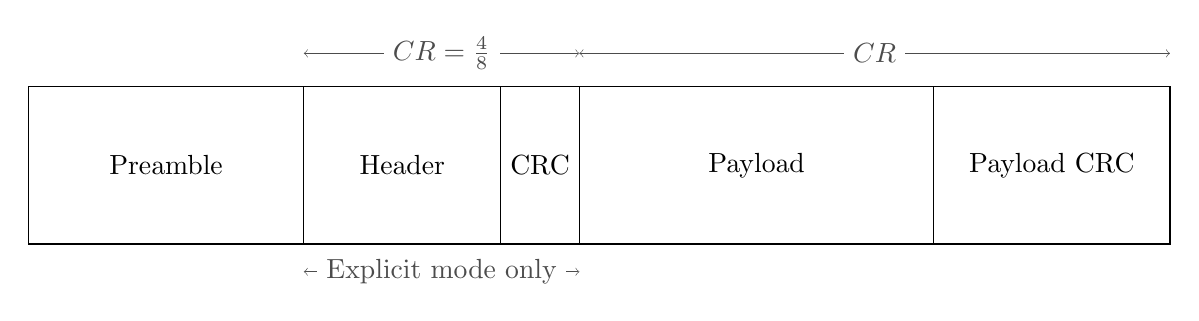
\begin{tikzpicture}[
  timeslot/.style={draw, rectangle, minimum size=1cm},
  description/.style={draw, rectangle, minimum size=1cm},
  arr/.style={help lines,black!70,<->},
]
\begin{scope}[xshift=0cm,yshift=0cm,inner sep=0pt, outer sep=0pt]
  \node (desc0) [description, fit={(0,0) (3.5,2)}, label=center:{Preamble}] {};
  \node (desc1) [description, fit={(3.5,0) (6,2)}, label=center:{Header}] {};
  \node (desc2) [description, fit={(6,0) (7,2)}, label=center:{CRC}] {};
  \node (desc4) [description, fit={(7,0) (11.5,2)}, label=center:{Payload}] {};
  \node (desc5) [description, fit={(11.5,0) (14.5,2)}, label=center:{Payload CRC}] {};
\end{scope}

\draw[arr]
  ([yshift=12pt]desc1.north west) -- node[fill=white] {$CR = \frac{4}{8}$} ([yshift=12pt]{desc2.north east});
\draw[arr]
  ([yshift=-10pt]desc1.south west) -- node[fill=white] {Explicit mode only} ([yshift=-10pt]{desc2.south east});

\draw[arr]
  ([yshift=12pt]desc4.north west) -- node[fill=white] {$CR$} ([yshift=12pt]{desc5.north east});
\end{tikzpicture}
\caption{LoRa Packet Structure\cite{semtech:sx}\label{fig:packetformat}}
\end{figure}

\begin{description}
  \item[Preamble] synchronizes the receiver for the incoming data flow. The
    preamble length is configurable.
  \item[Header] Depends on the packet type explicit or implicit.
  \begin{description}
    \item[Explicit] mode header provides information on the payload.
    \begin{itemize}
      \item Payload length in bytes.
      \item Forward Error Correction code rate.
      \item The presence or not of the payload cyclic redundancy check (CRC).
    \end{itemize}
    \item[Implicit] mode removes the header from the packet. This mode should be
      used when payload, coding rate, and CRC presence are known, and when we want to
      reduce the packet length.
  \end{description}
  \item[Payload] is a variable-length field containing the transmitted data as
    well as an optional CRC.
\end{description}

\subsection{Time on Air (ToA)}

The Time on Air is the measure for packet transmission time.
ToA depends on the parameters we introduced previously to count the number of
symbols that constitute each payload.

The following formula defines the duration of each symbol~\ref{eq:tsymlong}.
Equation~\ref{eq:tsym} is equivalent to the relation~\ref{eq:bw}.

\begin{equation}
  \label{eq:tsymlong}
  T_{sym} = \frac{1}{R_{sym}}
\end{equation}

\begin{equation}
  \label{eq:tsym}
  T_{sym} = \frac{2^{SF}}{BW}
\end{equation}

The ToA is the sum of the time to transmit the packet preamble and the packet
payload.

\begin{equation}
  \label{eq:tpacket}
  T_{packet} = T_{preamble} + T_{payload}
\end{equation}

Equation~\ref{eq:tpreamble} calculates the preamble time. The $n_{preamble}$
or preamble length is programmable.

\begin{equation}
  \label{eq:tpreamble}
  T_{preamble} = (n_{preamble} + 4.25)T_{sym}
\end{equation}

The following equation~\ref{eq:payloadsymnb} gives the number of symbols in the
payload of the packet.
The symbols number depends on the following parameters.

\begin{description}
  \item[PL] The payload length in bytes.
  \item[SF] The spreading factor.
  \item[H] Whether (0) or not (1) the header is enabled.
  \item[DE] Whether (1) or not (0) data rate optimization is enabled.
  \item[CR] The coding rate.
\end{description}

\begin{equation}
  \label{eq:payloadsymnb}
  n_{payload} = 8 + \max(ceil(\frac{8PL - 4SF + 28 + 16 - 20H}{4(SF - 2DE)})(CR + 4),0)
\end{equation}

The payload durations in~\ref{eq:tpayload} give the total packet time on-air
with~\ref{eq:tpacket}.

\begin{equation}
  \label{eq:tpayload}
  T_{payload} = n_{payload} T_{sym}
\end{equation}


\subsection{Channels}

% See 'Understanding the limits of LoRaWAN' the 3 channels definition in Europe
% The channels available is dependant on the country rules we are transmitting from.
The Things Network~\cite{ttnfrequencyplans} did a summary of the available
channels available depending on your frequency plan.

Figure~\ref{fig:channels} presents each LoRaWAN channel available in the
European ISM band (863-870 MHz)~\cite{Polonelli_2019}.

\begin{figure}[H]
  \centering
  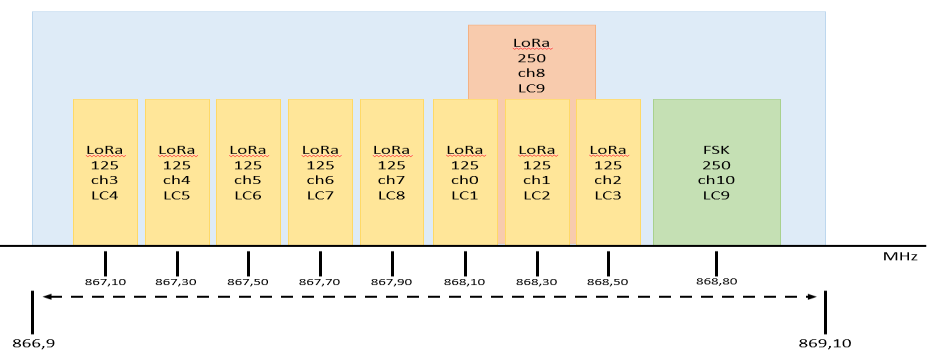
\includegraphics[width=\textwidth]{thesis.tex/chapters/context/fig/channels.png}
  \caption{LoRaWAN Channels in Europe\cite{Polonelli_2019}\label{fig:channels}}
\end{figure}

% TODO Talk about 1% duty cycle

\section{Time-Slotted Channel Hopping (TSCH)}

TSCH is a Medium Access Control (MAC) layer protocol defined by the IEEE
802.15.4e standard~\cite{rfc7554}.
The design is inherited from WirelessHART and
ISA100.11a~\cite{Duquennoy2017TSCHA6}.
Time synchronization aims to achieve low power and highly reliable
communications by using the following principles.

\begin{description}
  \item[Time-division multiple access] or (TDMA) by assigning time slots for each
    participant in the network avoiding collisions.
  \item[Synchronization] time-synchronized nodes syncing their clock with each
    other for being able to keep the notion of \emph{time slot}.
  \item[Channel Hopping] for better band usage, less interference, and more
    throughput.
\end{description}

In the following section I will present the TSCH protocol building blocks.

\subsection{Time Slots}

A time slot in TSCH is a unit of time to execute the network operations. 
The duration of the time slot is not standardized and depends on the physical 
layer we are using. 
Time slots should be long enough for the longest frame size to be sent
between two nodes, together with an acknowledgement~\cite{rfc7554}. 
Every time slot in a TSCH network has the same duration.

For each time slot operation, a schedule orchestrates what each
node of the network will use his time-slot for.

\begin{description}
  \item [Transmit] if a packet is on the outgoing buffer of the node.
  \item [Receive] listen for incoming packets that may arrive.
  \item [Sleep] to save energy.
\end{description}

Each transmitting or receiving time slot is made of the following parts.

\begin{itemize}
  \item The packet transmission or reception.
  \item Guard time for time slots synchronization.
  \item Acknowledgement reception or transmission.
\end{itemize}

\paragraph{}

A set of time slots that repeat over time is known as a slotframe.
A slotframe is made of time slots and empty slots.
The slotframe length has a direct impact on network capacity.
Figure~\ref{fig:timeslots} represents how time slots and slotframes are
organized together. 

\begin{figure}[H]
  \centering

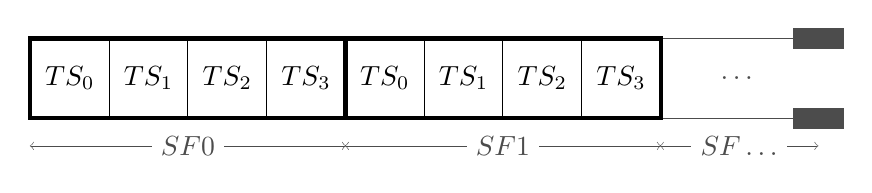
\begin{tikzpicture}[
  timeslot/.style={draw, rectangle, minimum size=1cm},
  arr/.style={help lines,black!70,<->},
]

\foreach [evaluate={\ts=int(mod(\i, 4))}] \i in {0,...,7} {
  \node (ts\i) [timeslot] at (\i, 0) {$TS_{\ts}$};
}
\node (ts8) [minimum height=1cm, minimum width=2cm, black!70] at (8.5, 0) {\ldots};
\draw[help lines, black!70]
  (ts8.north west) -- (ts8.north east) node[fill=white, black!70] {$\ldots$};
\draw[help lines, black!70]
  (ts8.south west) -- (ts8.south east) node[fill=white, black!70] {$\ldots$};

\draw[ultra thick] 
  (ts0.south west) rectangle (ts3.north east)
  (ts4.south west) rectangle (ts7.north east);

\draw[arr]
  ([yshift=-10pt]ts0.south west) -- node[fill=white] {$SF0$} ([yshift=-10pt]{ts3.south east});
\draw[arr]
  ([yshift=-10pt]ts4.south west) -- node[fill=white] {$SF1$} ([yshift=-10pt]{ts7.south east});
\draw[arr]
  ([yshift=-10pt]ts8.south west) -- node[fill=white] {$SF\ldots$} ([yshift=-10pt]{ts8.south east});

\end{tikzpicture}

\caption{Slotframes representation\label{fig:timeslots}}
\end{figure}


\subsection{Absolute Slot Number (ASN)}

The absolute slot number is a shared counter between all the devices that
define the number of time slots elapsed since the start of the
network (see Fig~\ref{fig:asn}).
ASN increases after each time slot and is calculated with \ref{eq:asn} where $k$
is the slotframe offset.

\begin{equation}
  \label{eq:asn}
  ASN = k SF_{len} + TS_{offset}
\end{equation}

\begin{figure}[H]
\centering
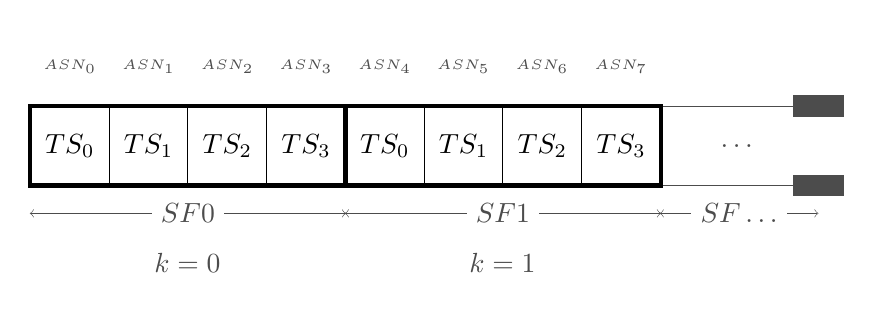
\begin{tikzpicture}[
  asn/.style={black!70, minimum size=1cm},
  timeslot/.style={draw, rectangle, minimum size=1cm},
  arr/.style={help lines,black!70,<->},
  desc/.style={black!70},
]

\foreach \i in {0,...,7} {
  \node (ts\i) [asn] at (\i, 1) {\tiny $ASN_{\i}$};
}
\foreach [evaluate={\ts=int(mod(\i, 4))}] \i in {0,...,7} {
  \node (ts\i) [timeslot] at (\i, 0) {$TS_{\ts}$};
}
\node (ts8) [minimum height=1cm, minimum width=2cm, black!70] at (8.5, 0) {\ldots};
\draw[help lines, black!70]
  (ts8.north west) -- (ts8.north east) node[fill=white, black!70] {$\ldots$};
\draw[help lines, black!70]
  (ts8.south west) -- (ts8.south east) node[fill=white, black!70] {$\ldots$};

\draw[ultra thick] 
  (ts0.south west) rectangle (ts3.north east)
  (ts4.south west) rectangle (ts7.north east);

\draw[arr]
  ([yshift=-10pt]ts0.south west) -- node[fill=white] {$SF0$} ([yshift=-10pt]{ts3.south east});
\draw[arr]
  ([yshift=-10pt]ts4.south west) -- node[fill=white] {$SF1$} ([yshift=-10pt]{ts7.south east});
\draw[arr]
  ([yshift=-10pt]ts8.south west) -- node[fill=white] {$SF\ldots$} ([yshift=-10pt]{ts8.south east});
\node[desc] at
  ([xshift=2cm, yshift=-28pt]ts0.south west) {$k = 0$};
\node[desc] at
  ([xshift=2cm, yshift=-28pt]ts4.south west) {$k = 1$};
\end{tikzpicture}
\caption{Absolute Slot Number\label{fig:asn}}
\end{figure}


\subsection{Channel Hopping}

\emph{Channel Hopping} increases the network capacity with frequency diversity
to mitigate interferences.
Multiple devices can share time slots to transmit at the same time on different
channels.

Links are the conjunction of a time slot and a channel~\cite{Chen2013PerformanceAO}.

\begin{equation}
  \label{eq:links}
  link = (TimeSlot_{number}, Channel_{offset})
\end{equation}

Multiple links constitute a time slot (dependent on the number of channels
available). Devices can transmit on different links during the same time slot.

% TODO Topology example multiple timeslot same time TX on different channels

The channel offset is computed by the transmitter and the receiver with the
function~\ref{eq:channel}. Both nodes know the $ASN$ and the schedule and can
compute the same channel offset~\cite{rfc7554}.

\begin{equation}
  \label{eq:channel}
  Channel_{offset} = (ASN + Scheduled_{offset}) \% Channel_{number}
\end{equation}

If the slotframe length is a prime number, even with the static schedule,
with known channel offset, the time slot will use a different channel every time.
Figure~\ref{fig:channelhopping} shows how scheduled cells in a TSCH network of
four time slots and three channels change channel depending on the ASN.

\begin{figure}[H]
\centering
\begin{tikzpicture}[
  asn/.style={black!70, minimum size=1cm},
  timeslot/.style={draw, rectangle, minimum size=1cm},
  arr/.style={help lines,black!70,<->},
  desc/.style={black!70},
]

\foreach \i in {0,...,7} {
  \node (asn\i) [asn] at (\i, 4) {\tiny $ASN_{\i}$};
}
\foreach [evaluate={\ts=int(mod(\i, 4))}] \i in {0,...,7} {
  \node (ts3\i) [timeslot] at (\i, 3) {};
}
\foreach [evaluate={\ts=int(mod(\i, 4))}] \i in {0,...,7} {
  \node (ts2\i) [timeslot] at (\i, 2) {};
}
\foreach [evaluate={\ts=int(mod(\i, 4))}] \i in {0,...,7} {
  \node (ts1\i) [timeslot] at (\i, 1) {};
}
\foreach [evaluate={\ts=int(mod(\i, 4))}] \i in {0,...,7} {
  \node (ts\i) [asn] at (\i, 0) {$TS_{\ts}$};
}
% \node (ts8) [minimum height=1cm, minimum width=2cm, black!70] at (8.5, 0) {\ldots};
% \draw[help lines, black!70]
%   (ts8.north west) -- (ts8.north east) node[fill=white, black!70] {$\ldots$};
% \draw[help lines, black!70]
%   (ts8.south west) -- (ts8.south east) node[fill=white, black!70] {$\ldots$};

\node (choff3) [black!70] at (-1.5, 3) {$Ch_{off} 2$};
\node (choff2) [black!70] at (-1.5, 2) {$Ch_{off} 1$};
\node (choff1) [black!70] at (-1.5, 1) {$Ch_{off} 0$};

\begin{scope}[on background layer]
\fill[blue!50] (ts10.south west) rectangle (ts10.north east);
\fill[blue!50] (ts24.south west) rectangle (ts24.north east);

\fill[orange!50] (ts30.south west) rectangle (ts30.north east);
\fill[orange!50] (ts14.south west) rectangle (ts14.north east);

\fill[green!50] (ts22.south west) rectangle (ts22.north east);
\fill[green!50] (ts36.south west) rectangle (ts36.north east);
\end{scope}

\draw[ultra thick] 
  (ts10.south west) rectangle (ts33.north east)
  (ts14.south west) rectangle (ts37.north east);

\draw[arr]
  ([yshift=-10pt]ts0.south west) -- node[fill=white] {$SF0$} ([yshift=-10pt]{ts3.south east});
\draw[arr]
  ([yshift=-10pt]ts4.south west) -- node[fill=white] {$SF1$} ([yshift=-10pt]{ts7.south east});
\draw[arr]
  ([yshift=-10pt]ts8.south west) -- node[fill=white] {$SF\ldots$} ([yshift=-10pt]{ts8.south east});
\node[desc] at
  ([xshift=2cm, yshift=-28pt]ts0.south west) {$k = 0$};
\node[desc] at
  ([xshift=2cm, yshift=-28pt]ts4.south west) {$k = 1$};
\end{tikzpicture}
\caption{Two slotframes with scheduled cells changing channel between slotframes\label{fig:channelhopping}}
\end{figure}


\subsection{Scheduling}

The TSCH schedule tells each node what to do during a time slot.

Dedicated time slots cells need the following parts to be defined.

\begin{itemize}
  \item Receive or transmit.
  \item The channel offset.
  \item Address of the node to communicate with.
\end{itemize}

% Shared cells multiple nodes can transmit at the same time on the same channel.

To ensure the execution of the same slots, each transmission is an opportunity 
for the neighbor to resynchronize their clocks.
Synchronization is important to mitigate each node internal clock drift.

Time source nodes send Enhanced Beacon (EB) packets to synchronize the receiving
nodes of the network. When nodes don't resynchronize for a long period
a Keep-Alive (KA) is sent and used to adjust the drift at synchronization.

Figure~\ref{fig:sync} represents the clock drift that can occur between two
distant time slots.
As we can see the receiver will know the drift based on the moment he receives
the data and then adjusts its time slot length to finish earlier.

\begin{figure}[H]
  \centering
  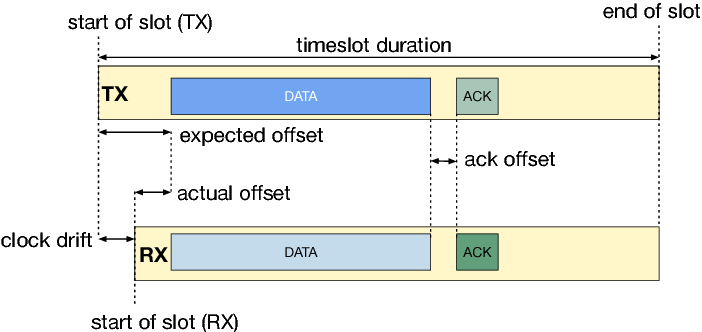
\includegraphics[width=\textwidth]{thesis.tex/chapters/context/fig/sync.png}
  \caption{Synchronization in a TSCH time slot\cite{TELESHERMETO201784}\label{fig:sync}}
\end{figure}

\section{Routing}

Because I will use two different routing protocols in
Chapter~\ref{section:tsch} to prove my implementation worked, I will introduce
in this section RPL and Orchestra.
This section is not meant to be an in depth explanation of the protocols.
Giving such details would be out of the scope of my work as I don't modify any
of the components of those protocols.

\subsection{Routing Protocol for Low-Power and Lossy Networks (RPL)}

RPL is a routing protocol for constrained device networks.
It means RPL can work on network with high data loss rates, low data rates and
instability~\cite{rfc6550}.

The routing in RPL is based on Destination Oriented Directed Acyclic Graphs (DODAG).
All the nodes of the DODAG are routed toward the \emph{root} node. 
If the root node is connected to internet it can be used as a \emph{border
router}.
RPL give each node a rank based on the distance from the root node, calculated
with an \emph{objective function}.
The routing between nodes in RPL is based by sending packets up to a smaller 
ranked parent until it reach a common ancestor and then sending the packet down
to the destination~\cite{duquennoy2015}.

\subsection{Orchestra}

Orchestra is a scheduler that work on top of TSCH+RPL
networks where each node autonomously compute their own schedules without the
need of a scheduler~\cite{duquennoy2015}.
Each node maintain their own schedule and keep track of their neighbor solely
on the network information from RPL.
Orchestra maintain different slotframes for these different network operations

\begin{itemize}
  \item Application data
  \item RPL traffic
  \item TSCH beacon
\end{itemize}

By using mutually prime slotframe length to avoid overlap and computing time
and channel offset using the sender and receiver identification as parameter,
Orchestra achieve very low level of collisions~\cite{duquennoy2015}.

\section{Contiki OS}

Contiki is a free and open-source Real-Time operating system (OS) specifically made
for IoT applications. Contiki ships with a low-power IPv6 communication stack
and a variety of routing and MAC protocols making the OS particularly well
suited for Wireless Sensor Networks (WSN).

Contiki uses protothreads, a programming abstraction which Contiki is
built around.
They allow developers to write event-driven programs with little memory overhead and
claims to reduce the complexity of embedded programs that used to be written 
like state machines~\cite{10.1145/1182807.1182811}.

The Contiki OS project has been unmaintained since 2017 but its
successor named Contiki-NG was created as a fork by the same developers since.
That fork has been the basis for a lot of LPWAN experimentation, for example 
with the development of the 6TiSCH stack for the OS~\cite{Duquennoy2017TSCHA6}.

\paragraph{}

Contiki's Network Protocol stack, also known as \lstinline{NETSTACK}, is a
feature of the OS.
It allows developers to defines parts of the network stack we are using in a Contiki
project (Fig~\ref{fig:netstack}).

NETSTACK implementation allows Contiki to communicate between layers without 
knowing the specific implementation of the layer.
Developers must define the following variables to change the network stack 
in a Contiki project.

\begin{itemize}
  \item \lstinline{NETSTACK_NETWORK}
  \item \lstinline{NETSTACK_ROUTING}
  \item \lstinline{NETSTACK_MAC}
  \item \lstinline{NETSTACK_RADIO}
\end{itemize}

\begin{figure}[H]
\centering
  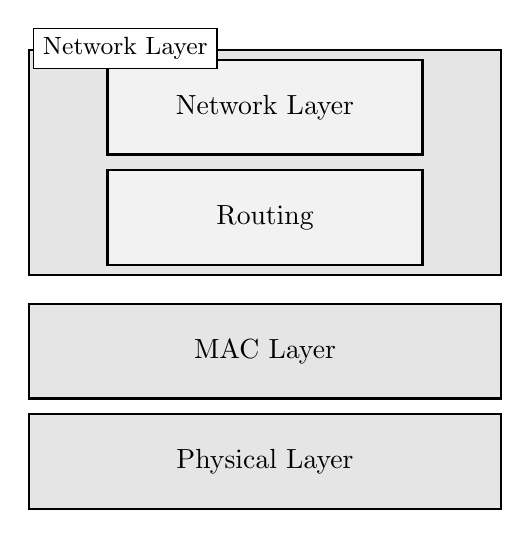
\begin{tikzpicture}[->,>=stealth',shorten >=1pt,auto,node distance=1.4cm]

  \tikzstyle{comment}=[
    right=2pt,
    font=\small,
    fill=white,
    text=black,
    draw=black,
  ]

  \tikzstyle{every state}=[rectangle,thick,
    draw=black,fill=gray!20,text=black,
    minimum width= 6cm,
    minimum height= 1.20cm
  ]

  \tikzstyle{smallstate}=[rectangle,thick,
    draw=black,fill=gray!10,text=black,
    minimum width= 4cm,
    minimum height= 1.20cm
  ]

  \node[smallstate]         (A)                    {Network Layer};
  \node[smallstate]         (B) [below of=A]       {Routing};
\begin{scope}[on background layer]
  \node[state, fit=(A)(B)] (AB)                 {};
\end{scope}
  \node[state,below=1cm]         (C) [below of=AB]       {MAC Layer};
  \node[state]         (D) [below of=C]       {Physical Layer};

  \node[comment]       at (AB.north west) {Network Layer};
  % \node[comment]       at (C.north west) {MAC Layer};
  % \node[comment]       at (D.north west) {Physical Layer};
  % \path (A) edge [bend right]    node {     } (B)
  %           edge [bend left]     node {     } (C)
  %       (B) edge [bend left]     node {     } (C)
  %           edge                 node {     } (D)
  %       (C) edge [bend left]     node {     } (A)
  %       (D) edge [bend right=85] node {     } (A);
\end{tikzpicture}
\caption{The Contiki's Network Protocol Stack\label{fig:netstack}}
\end{figure}


\section{Related work}

This is not the first attempt to bring multi-hop communication to LoRa.
This section will give a state of the art of the research on
multi-hop routing in LoRa.

\paragraph{}

Work to port TSCH and the 6LoWPAN stack to a new radio protocol has already 
been done in~\cite{uwbtsch} for the Ultra-Wide Band (UWB).

% \paragraph{BLEach}

\paragraph{UWB-TSCH}

Charlier M. in~\cite{uwbtsch} explores the requirements to adapt TSCH for the UWB.
Similarly to LoRa, UWB does not allow CCA and can not use CSMA for its 
communications.
His work shows what it takes to adapt TSCH for another radio layer. 
It is also an evaluation of the performance of TSCH outside of 802.15.4.

\paragraph{}

The respective authors of~\cite{DIAS2018424, 8856256}, look at ways to extend
the current LoRaWAN MAC protocol to allow multi-hop communications.

\paragraph{Multihop LoRaWAN Extension} Dias J., Grilo A. in \cite{DIAS2018424}
design a routing protocol that can interoperate with LoRaWAN gateways while
using multi-hop communications for nodes out of the range of the gateway.  
The extension uses beacons to achieve time synchronization, but no channel
hopping is used.

% \paragraph{Distributed Queuing (DQ) LoRa}

% The authors of~\cite{8856256} extend LoRaWAN

% \subsection{RS LoRa}
% [18] in roald similar to lorawan extension
% \subsection{Listen before talk LoRa}
% [17] in roald work

\paragraph{}

Studies on creating a new MAC protocol for multi-hop LoRa communications in a linear
network has been done in~\cite{Abrardo_2019,duong2018}.

\paragraph{Linear Multihop LoRa}

Abrardo A. and Pozzebon A.~\cite{Abrardo_2019} studied the deployment of a
large scale LoRa network to monitor the underground medieval aqueducts of the city center 
of Sienna, the \emph{Bottini}.

Because of the large deployment cost induced by the large tunnels, the negative 
aesthetic impact of a wired network and the risk of flooding, made the author
opt for a battery-operated wireless network.


They propose a multi-hop routing solution for Linear Sensor Network (LSN) based 
on LoRa by developing their own MAC protocol tailored for their scenario.
This custom protocol is built around assigning time slots for each node with
a common schedule for adjacent nodes.
This allows neighbors to synchronize their clock and broadcast messages to
both ends of the aqueducts.

% Their solution allowed the connection of the Bottini

\paragraph{Multi-Hop Linear Network Based on LoRa}

Duong T. in~\cite{duong2018} proposes a multi-hop protocol for LoRa linear
networks. 
His network is made of two periods. The first is the network initialization to
verify the gateway is reachable and synchronizes the nodes to make them join the 
data operation period.
Each node transmits in a different time slot to their parent node, each hop adds
their information to the packet they are relaying until the gateway is
reached.
The clock drift is mitigated by synchronizing on the preamble but the receiver
does not acknowledge the reception of the packet, making the network sensible to
interference since it is running on a single channel and SF.

\paragraph{}

The next studies look at ways to create a fully functioning multi-hop network
using LoRa without depending on LoRaWAN specifications.

\paragraph{LoRaBlink}

Bor M., Vidler J., Roedig Utz. in \cite{lorablink} propose the LoRaBlink
protocol, designed to support reliable and energy efficient multi-hop
communication.

Each node of the network remains in listening mode until a beacon is received.
Beacons are used for time synchronization of the time slots.
Each node transmits packets to their parent node that relays it to the gateway.
There is no scheduling of which node transmits, two nodes may
transmit at the same time.

% Every nodes of the network keep track of their distance to the sink

Also, LoRaBlink uses fixed SF, BW, and channel. This decreases the overall throughput 
of the network and makes it highly sensitive to interference.

\paragraph{RPL+LoRa MAC Protocol}

The Authors of~\cite{8115756} from the SmartNet research group of VUB, adapted RPL 
to enable multihop communications on top of LoRa. 
The paper presents the modifications of the objective function to take into
account the SF when computing the best routes.
The paper describes a solution for a network of nodes to discover each other.
It uses a router sending packets on different spreading factors while the joining
node listens on the spreading factors by starting by the lowest, this way it
picks the fastest spreading factor available.
It also describes a custom MAC protocol, \emph{RLMAC}, to allow multi-hop
routing with LoRa. It manages time slots between nodes and allows PHY settings
tuning depending on the links.

The protocol proposed focused on having the fastest delivery time with LoRa
communications while increasing the packet delivery rate (PDR).
Reducing the power consumption was not a concern in this paper.


\paragraph{TSCH-over-LoRa}

In the course of my work, a new study from Haubro M., Orfanadis C.,
Oikonomou G. and Fafoutis X.~\cite{tschoverlora} came out on the exact 
same subject as mine. 
Their work studied the feasibility of porting TSCH to LoRa in Contiki OS using
the SX1272 radio module.

The authors proved it was possible to adapt TSCH for LoRa by testing their
implementation with a variety of routing protocols and applications.
Their implementation works on a single SF at a time but they tested it using
SF7 and SF10.

To demonstrate the resilience of TSCH to interference even with LoRa, the
authors made a radio jammer that transmits on different channels. Their
experimentation proved no packets got lost when using channel hopping with
LoRa.


\chapter{Radio Driver for Zolertia with the RN2483 module\label{section:radio}}

% Most of the LoRaWAN features were not implemented or tested since this was out of the scope of this project.

The \emph{Zolertia RE-Mote REV-B} platform doesn't support \emph{LoRa} out of
the box. This chapter covers the implementation of a radio driver on
\emph{Contiki-NG} for the \emph{RN2483}, a LoRa module from Microhip,
communicating with the \emph{RE-Mote} platform.

\section{Preliminary work}

Last year \emph{Roald Van Glabbeek}, in the course of his master thesis~\cite{8847137}, 
aiming on doing further research on \emph{energy efficient lora multihop networks}, 
started working on the \emph{RN2483} module.
For this purpose he made \emph{RN2483 Shields} adapted to the pin
configuration of the \emph{Zolertia RE-Mote REV-B}. He also started a radio driver
implementation for Contiki-OS\@.

In a previous attempt to adapt \emph{TSCH} for \emph{LoRa}
in~\cite{njomgang_2018}, Serge did his experimentation with the \emph{LoRaMote}
demo platform from \emph{Semtech} using a different LoRa radio module the
\emph{SX1272}. 
As analyzed in~\cite{8847137}, LoRaMotes turned out to be an issue for the
further research because they were no longer produced, 
new versions were expensive and memory was a bottleneck.
That's why \emph{Zolertia RE-Mote} was chosen. The platform is already available 
and well maintained in \emph{contiki-ng} (making the transition faster and less
error prone as less code need to be developed) and the platform was already used 
in the \emph{ETRO Lab}.

The first part of my work consisted in implementing a reliable
and fully featured radio driver for the \emph{RN2483} module working in the last
version of \emph{contiki-ng}.

\section{RN2483 Module Structure}

Developed by \emph{Microchip} the \emph{RN2483} is a LoRa module operating in
the 433 MHz and 868 MHz Frequency Bands~\cite{microchip:rn2483}. 
The module is specifically designed to work with LoRaWAN compatible networks, 
by including a set of commands designed for seamless integration with the
\emph{LoRaWAN Protocol Stack}

All communication to and from the module are done via \emph{UART} ASCII command,
making it easy for a human to interact with the module by handwriting commands
on a terminal and reading the response back in a readable format
(see~\ref{fig:pconn}).
% The module is made for ease of use over performance and power consumption.

\begin{figure}[H] % TODO More info on axis
\centering
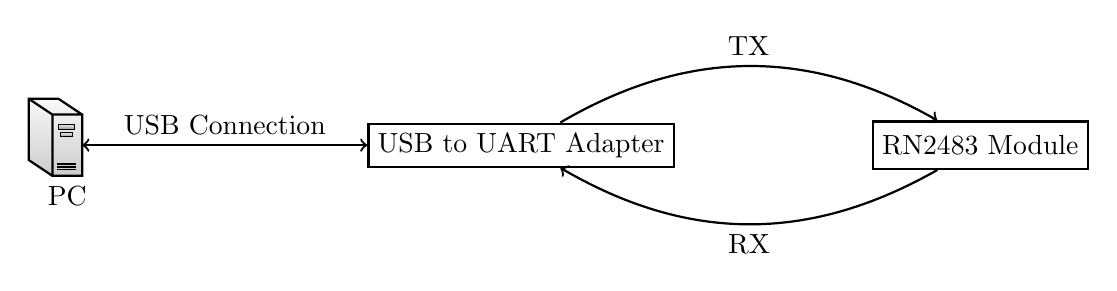
\begin{tikzpicture}[auto, thick]
  \node(pc) [server, label=below:{PC}] {};
  \node(ftdi) [draw, rectangle, right=of pc, right=4cm] {USB to UART Adapter};
  \node(module) [draw, rectangle, minimum size=6mm, right=of ftdi, right=2.5cm] (module) {RN2483 Module};

  \path (pc) edge[<->] node[]{USB Connection} (ftdi) ;
  \path (ftdi) edge[->,bend left] node[text width=1cm, align=center]{TX} (module);
  \path (module) edge[->,bend left] node[text width=1cm, align=center]{RX} (ftdi);
\end{tikzpicture}
\caption{Simple communication with the module scenario\label{fig:pcconn}}
\end{figure}


The module's interface include three types of commands that enable access to
different functions~\cite{microchip:reference}.

\begin{itemize}
  \item \emph{radio} for the low-level radio commands to access the transceiver
    and PHY settings directly without the LoRaWAN interface overhead.
  \item \emph{mac} to access the LoRaWAN protocol stack configurations and
    commands. This command set will be used less as our implementation require 
    low-level transceiver access.
  \item \emph{sys} for the module specific configurations such as the module
    GPIOs state, \emph{sleep}, EEPROM memory access, \ldots
\end{itemize}

\section{Testing Setup}

My testing setup was the same as~\cite{8847137}. I used a Zolertia RE-Mote
Rev-B platform, using the CC2538 microcontroller, connected to a
RN2483 breakout board, as schematized in Fig~\ref{fig:schemaconn}. 

The RE-Mote platform has two UART peripheral and we are using the UART1 peripheral 
to communicate with the module instead of UART0, already used by the platform USB 
debugger.

The reset pin of the module was wired to the \lstinline{PD0} GPIO to allow
software reset of the module as well as a push button for hard reset.

\begin{figure}[H]
  \centering
  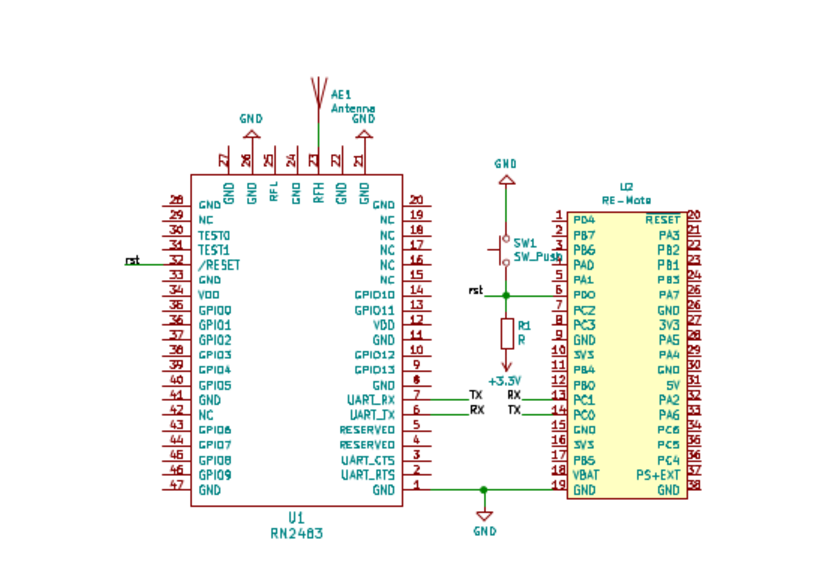
\includegraphics[scale=0.70]{thesis.tex/chapters/driver/fig/conn_diag.pdf}
  \caption{Hardware connection\label{fig:schemaconn}}
\end{figure}

\section{Implementation}

All the files for the driver implementation are available in
\lstinline{/arch/dev/rn2483} and examples are located in
\lstinline{/examples/platform-specific/rn2483}.

\subsection{Structure}

My implementation structure was inspired by the work in~\cite{8847137} as well
as the \emph{RIOT-OS} project\footnote{\url{https://github.com/RIOT-OS/RIOT}}, which
already took care to define a lot of the parameters we want to use with the
module.

Following, is a listing of the different files I created and their usage.

\begin{description}
  \item[lora] LoRa radio specific functions, declaration and configuration. This
    include functions used to calculate the time on air as well as
    LoRa PHY configuration structure and parameters.
  \item[rn2483-include] This file contain the declaration both needed by
    \lstinline{rn2483-uart} and \lstinline{rn2483} to avoid cycling inclusion
    that mess with the compiler.
  \item[rn2483-uart] Lower level implementation of the function to directly
    communicate with the module via UART\@. This part is the closest one to the
    hardware because of the uart implementation being specific to the CC2538.
  \item[rn2483-api] Complete coverage of the RN2483 commands. Using functions
    from this file allow the user of the driver to not bother writing
    each command by hand and use a standardized structure instead.
  \item[rn2483] Implementation of the Contiki radio device driver. The file
    contain the standardized way of Contiki to use and configure a radio device.
    This is the structure shared by all the radio driver in Contiki.
\end{description}

\subsection{Synchronous communication with the module}

The first design challenge of the driver implementation is to create a
synchronous mechanism to receive message from the UART\@. 
The need for synchronous messaging is crucial since every
transmission, configuration and reception are done via UART\@.
Acknowledgements from commands are mandatory to avoid command
clash when trying to use the module at the same time.
The previous implementation in~\cite{8847137} used fixed time delays to 
wait for the command to be fully executed on the module. However, this method 
quickly showed its own limitation, each commands has their own delays and a
fixed delay slow down the global execution.

% TODO Maybe sequence diagram with a clash

The UART driver implementation for the CC2538 in Contiki don't have a synchronous 
blocking read function out of the box, it assume the programmer will compute the
responses from UART in processes instead by waiting for event instead.
The way the reception is working is by executing a so called \emph{input handler} 
at each interruption triggered by UART reception.
The default input handler is the \lstinline{serial_line_input_byte} 
specifically designed for serial communication with a terminal and we will keep
using this handler with UART0 to get debug messages with a USB connection from 
a computer.

However, we have to define our own handler for the UART1 peripheral directly
connected with the module.
It will be similar as the default one because they are both using same message
structure terminating by \lstinline{\r\n}, but 
where \lstinline{serial_line_input_byte} is passing each character to a standalone
process (called \lstinline{serial_line_process}) broadcasting an event when the 
command is fully received, our handler is directly threating the message in the 
interrupt.

Working with processes and events, is not possible in our use case because Contiki 
don't have any mechanisms allowing programmers to wait for an event inside a 
function. Instead, Contiki allow to only wait for specific events inside
processes, but doing everything inside a big process is not an option.
The custom handler is designed as a state machine (Fig~\ref{fig:cmdstate}) and 
work with its own reception buffer. It takes advantage of the limited response 
format from the RN2483 module to sort each new communications.

\begin{itemize}
  \item Messages starting with \lstinline{radio rx  } are asynchronous LoRa
    radio messages.
  \item \lstinline{radio_tx_ok} indicate the end of a radio transmission. This
    implies we have done a transmission before.
  \item \lstinline{ok} indicate the acknowledgement of a command.
\end{itemize}

% Talk about the state machine

I implemented helper functions, to ease the command transmission and
acknowledgement between the RE-Mote and the RN2483.

\begin{description}
  \item[rn2483\_receive\_synch] busywait on the command states
    (Fig~\ref{fig:cmdstate}) until the \emph{received} state is 
    reached, or after the timeout has elapsed.
  \item[rn2483\_send\_cmd] a \emph{printf} style command, automatically 
    waiting for acknowledgement (with the possibility to add a custom timeout).
  \item[rn2483\_raw\_cmd] sending the command from a buffer in argument
    without formatting or waiting for acknowledgement.
\end{description}

\begin{figure}[H]
\centering
  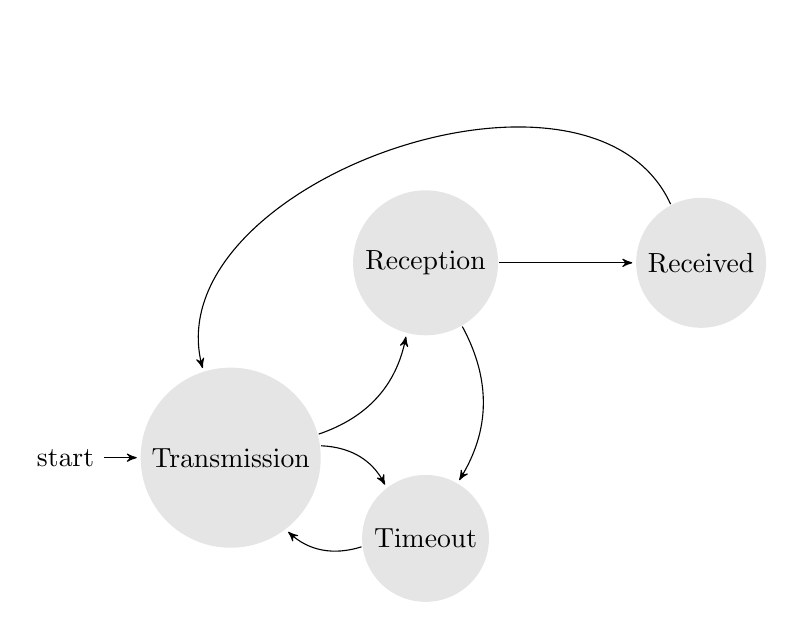
\begin{tikzpicture}[->,>=stealth',shorten >=1pt,auto,node distance=3.5cm]
  \tikzstyle{every state}=[thick,draw=gray!50,fill=gray!20,draw=none,text=black]

  \node[initial,state] (A)                    {Transmission};
  \node[state]         (B) [above right of=A] {Reception};
  \node[state]         (C) [below of=B]       {Timeout};
  \node[state]         (D) [right of=B]       {Received};

  \path (A) edge [bend right]    node {     } (B)
            edge [bend left]     node {     } (C)
        (B) edge [bend left]     node {     } (C)
            edge                 node {     } (D)
        (C) edge [bend left]     node {     } (A)
        (D) edge [bend right=85] node {     } (A);
\end{tikzpicture}
\caption{The command states\label{fig:cmdstate}}
\end{figure}


\subsection{Transmission}

The radio transmission command has a different pattern from the other commands 
of the module. After the acknowledgement of the radio transmission 
command (\lstinline{radio tx ...}) the module will also send a second message
when the message is fully transmitted.

\begin{figure}[H]
\centering

\begin{sequencediagram}

\newthread{A}{RE-Mote}{}
\newinst[1]{B}{RN2483}{}
\newinst[3]{C}{Radio Band}{}
\begin{call}{A}{radio tx~\ldots}{B}{radio\_tx\_ok}
  \messdash{B}{ok}{A}
  
  \begin{sdblock}{Radio Transmission}{Transmition time calculated
    in~\ref{eq:tpacket}}
    \begin{call}[4]{B}{}{C}{}
    \end{call}
  \end{sdblock}
\end{call}

\end{sequencediagram}

  \caption{\lstinline{radio tx} command sequence diagram\label{fig:txsequence}}

\end{figure}



Microchip chose to represent the payload as string formatted hex number to
facilitate the manual writing of commands, making the message payload twice as
long as its original content. As all the content we will handle 
are represented as \emph{8 bit} number array, a function to convert array to
string representation and vice versa was taken from the RIOT-OS project.

\subsection{Asynchronous Reception}

The last component of a complete driver implementation is to receive radio
messages.
Reception follow a different scheme from the other commands, a message
reception can happen at any time asynchronously from the moment we run the
command \lstinline{radio rx 0}.
To tackle this issue a one message inbox has been implemented (see
Fig~\ref{fig:rxstate}).
At the reception of a command from the module we look at the structure of
the message.
Every message coming from a radio communication start with \lstinline{radio rx  }, 
if it follow this structure a flag is set and is unset at the moment we read the
message from our code.
Messages are received in a string formatted hex number, we must convert it to an
\emph{8 bit integer array}. 
% TODO Talk about packet buf ?
% We don't store the final result in the same buffer as the one used for
% reception as reading the result 
% This array is stored in a different place than the received message as command
% may be executed between the moment we receive the message and the moment we
% read it.
Also, a timestamp is saved at the reception to keep track of when was received the
message.

\begin{figure}[H]
\centering
  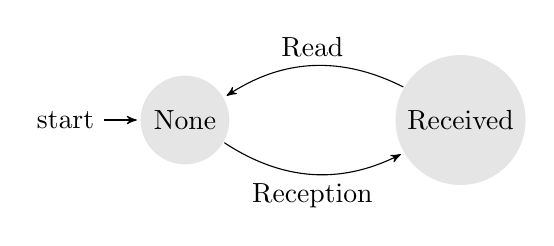
\begin{tikzpicture}[->,>=stealth',shorten >=1pt,auto,node distance=3.5cm]
  \tikzstyle{every state}=[thick,draw=gray!50,fill=gray!20,draw=none,text=black]

  \node[initial,state] (A)              {None};
  \node[state]         (B) [right of=A] {Received};

    \path (A) edge [bend right] node[below] {Reception} (B)
          (B) edge [bend right] node[above] {Read} (A);
\end{tikzpicture}
\caption{The RX states\label{fig:rxstate}}
\end{figure}


\subsection{Contiki Radio Driver}

The Contiki wiki didn't provided any information about writing our own radio driver
or porting a new radio platform for Contiki.
I based my implementation on the other radio driver implementation already
available on Contiki to understand the driver structure.

To create a Contiki radio driver we have to implement a \lstinline{radio_driver}
structure that must implement the following functions.

\begin{description}
  \item[init] is the first function of the driver executed at startup.
    This is where the configuration of the RN2483 take place
    as well as setting the module into point-to-point mode to not use the default
    LoRaWAN stack.
  \item[prepare] is the function called before a transmission with the data we
    want to transmit as parameter. 
    We can't transmit radio messages while listening for incoming messages, the
    first step of preparation is to exit the radio reception mode with the
    command \lstinline{radio rxstop}.
    The command also take care to convert the data to the hex string and
    already format the radio command ready to be sent.
  \item[transmit] send the already formatted command in the prepare function and
    wait for the \lstinline{radio_tx_ok} acknowledgement.
  \item[send] is the combination of prepare and transmit.
  \item[read], when a new message is received in the inbox, copy the radio
    message to the buffer passed in argument.
  \item[channel\_clear]
  \item[receiving\_packet] should theoretically check if the radio module is
    currently getting a new message from a transmission. This is a function we
    can expect from some platform with integrated radio module but here the
    simplicity of the RN2483 show his limit and I found no way for the module
    to acknowledge when it's receiving a new message.
  \item[pending\_packet] check the message inbox to see if we received a new
    message.
  \item[on] wake-up the module and start listening to radio messages.
  \item[off] stop listening to radio messages and put the module to sleep.
  \item[get\_value, set\_value, get\_object, set\_object] are all function used
    to configure the radio driver in a streamlined way. The parameter we need to
    implement will be discussed in Chapter~\ref{section:tsch}.
\end{description}

% TODO talk about Poll mode

\section{Validation test}

% Talk about project configuration like with the NETSTACK

To verify the implementation of the radio driver two examples were made.

\begin{itemize}
  \item The \emph{RN2483 shell} available in
    \lstinline{/example/platform-specific/lora/rn2483} is a tool to interact
    directly with the module.
  \item The \emph{ping-pong} example based on the nullnet example already
    available in \emph{contiki-ng} located in 
    \lstinline{/example/platform-specific/lora/nullnet} demonstrate the driver
    is correctly working with upper layer of the network stack.
\end{itemize}

For each Contiki project, the different OSI layers are defined using the
\emph{Contiki's Network Protocol stack}, or \lstinline{NETSTACK}, to select
each layer specific implementation we want to use in our project (Fig~\ref{fig:netstack}).
Also, each project are usually bundled with a \lstinline{project-conf.h}
configuration file where we can define the parameter of our project. 
To set my LoRa driver as the physical layer implementation we must add this line to
each \lstinline{project-conf.h}.

\begin{lstlisting}
#define NETSTACK_CONF_RADIO                        rn2483_radio_driver
\end{lstlisting}

\begin{figure}[H]
\centering
  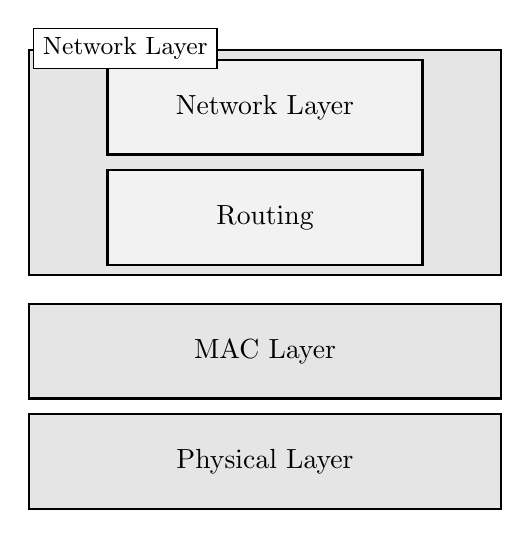
\begin{tikzpicture}[->,>=stealth',shorten >=1pt,auto,node distance=1.4cm]

  \tikzstyle{comment}=[
    right=2pt,
    font=\small,
    fill=white,
    text=black,
    draw=black,
  ]

  \tikzstyle{every state}=[rectangle,thick,
    draw=black,fill=gray!20,text=black,
    minimum width= 6cm,
    minimum height= 1.20cm
  ]

  \tikzstyle{smallstate}=[rectangle,thick,
    draw=black,fill=gray!10,text=black,
    minimum width= 4cm,
    minimum height= 1.20cm
  ]

  \node[smallstate]         (A)                    {Network Layer};
  \node[smallstate]         (B) [below of=A]       {Routing};
\begin{scope}[on background layer]
  \node[state, fit=(A)(B)] (AB)                 {};
\end{scope}
  \node[state,below=1cm]         (C) [below of=AB]       {MAC Layer};
  \node[state]         (D) [below of=C]       {Physical Layer};

  \node[comment]       at (AB.north west) {Network Layer};
  % \node[comment]       at (C.north west) {MAC Layer};
  % \node[comment]       at (D.north west) {Physical Layer};
  % \path (A) edge [bend right]    node {     } (B)
  %           edge [bend left]     node {     } (C)
  %       (B) edge [bend left]     node {     } (C)
  %           edge                 node {     } (D)
  %       (C) edge [bend left]     node {     } (A)
  %       (D) edge [bend right=85] node {     } (A);
\end{tikzpicture}
\caption{The Contiki's Network Protocol Stack\label{fig:netstack}}
\end{figure}


\subsection{Shell}

This example extend the existing shell available in Contiki by writing a set
of commands to test and interact with the the RN2483 via UART\@.

Here is the list of the added commands to the Contiki shell.

\begin{lstlisting}
'> sys': Send a 'system' command to the RN2483 Module.
'> mac': Send a 'mac' command to the RN2483 Module.
'> radio': Send a 'radio' command to the RN2483 Module.
'> tx': Transmit a radio message with the RN2483.
'> sleep': Put RN2483 into sleep mode.
'> wakeup': Force wakeup of RN2483.
'> rn2483_reset': Hardware Reset of the RN2483 Module.
'> help': Shows this help.
\end{lstlisting}

This was used during the development of the driver as a way to test parameters
as well as the synchronous communication implementation.

\subsection{Ping-Pong}

I based this example on the \emph{nullnet-broadcast} example to test if two
node could communicate using the LoRa driver I implemented when controlled by
the \emph{CSMA} MAC layer instead of directly using the driver API\@.

The example is using the NETSTACK in Fig~\ref{fig:pingpongstack}.

\begin{figure}[H]
\centering
  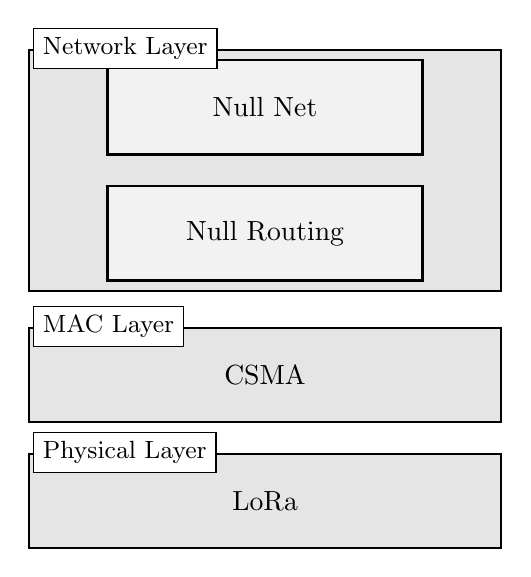
\begin{tikzpicture}[->,>=stealth',shorten >=1pt,auto,node distance=1.6cm]

  \tikzstyle{comment}=[
    right=2pt,
    font=\small,
    fill=white,
    text=black,
    draw=black,
  ]

  \tikzstyle{every state}=[rectangle,thick,
    draw=black,fill=gray!20,text=black,
    minimum width= 6cm,
    minimum height= 1.20cm
  ]

  \tikzstyle{smallstate}=[rectangle,thick,
    draw=black,fill=gray!10,text=black,
    minimum width= 4cm,
    minimum height= 1.20cm
  ]

  \node[smallstate]         (A)                    {Null Net};
  \node[smallstate]         (B) [below of=A]       {Null Routing};
\begin{scope}[on background layer]
  \node[state, fit=(A)(B)] (AB)                 {};
\end{scope}
  \node[state,below=1cm]         (C) [below of=AB]       {CSMA};
  \node[state]         (D) [below of=C]       {LoRa};

  \node[comment]       at (AB.north west) {Network Layer};
  \node[comment]       at (C.north west) {MAC Layer};
  \node[comment]       at (D.north west) {Physical Layer};
  % \path (A) edge [bend right]    node {     } (B)
  %           edge [bend left]     node {     } (C)
  %       (B) edge [bend left]     node {     } (C)
  %           edge                 node {     } (D)
  %       (C) edge [bend left]     node {     } (A)
  %       (D) edge [bend right=85] node {     } (A);
\end{tikzpicture}
\caption{The network stack used for the ping-pong example\label{fig:pingpongstack}}
\end{figure}


The example is a simple two-way communication between two RE-Motes. 
The first one is sending a request with a number as
payload and wait for the acknowledgement from the second motes sending back
the same payload. 
No other request is sent until the acknowledgement is received.
This is schematized in Fig~\ref{fig:pingpongsequence}.

The two different implementation to setup on each nodes are available in the
example folder.

\begin{itemize}
  \item \lstinline{ping.c} send the request and wait for acknowledgement.
  \item \lstinline{pong.c} send the acknowledgement.
\end{itemize}

\begin{figure}[H]
\centering

\begin{sequencediagram}

\newthread{A}{Mote A}{}
\newinst[1]{B}{Mote B}{}

\begin{call}[4]{A}{ping}{B}{pong}
\end{call}
\end{sequencediagram}

\caption{Description of the execution of the ping-pong example\label{fig:pingpongsequence}}

\end{figure}




\chapter{Time-Slotted Channel Hopping Implementation for LoRa\label{section:tsch}}

\section{Porting TSCH}

\subsection{Channels}

\subsection{Timestamp}

\subsection{Radio delay}

\subsection{$\mu s$ and rtimer ticks conversion}

\subsection{LoRa Time On Air}

\section{Adaptation of the timing}

\paragraph{Timing size issue}

\section{Testing}

\section{Considerations}


\chapter{Conclusion and further work}

The goal of the thesis was to adapt TSCH to work with LoRa to have a low power
and reliable multihop solution for LoRa using Contiki OS and the RN2483 LoRa
module.
% My work was built upon the previous work of student conducted in VUB but
% didn't achieved a fully working TSCH protocol working with LoRa.

\paragraph{}

My work was divided in two parts. 
In the first part I successfully implemented a working driver for the RN2483
module, the section~\ref{section:pingpong} detail how I ran a ping pong
example based on that driver.

The second part should have been limited to the adaptations of some variable 
of the TSCH protocol to work with LoRa.
But it turned out the long delay in LoRa communication made me discover a lot of
bugs coming from the current implementation of TSCH.

In his last year master thesis, Roald Van Glabbeek suggested further research
should conduct a power analysis on the RN2483 module.
I responded to this statement in~\ref{section:energyconsumption} about how
achieving a low power network with TSCH and this module is impossible because
of a missing feature.

The good news is I'm confident about achieving low power transmission with the
SX1272 module.
This thesis showed the way on what it take to adapt TSCH for a new radio
driver and re-implementation of this project with a module like SX1272 will then be
facilitated and would allow to measure meaningful data.
Questions and analysis of the accuracy of the network will then be possible.
A study of how longer sleeping period between de-synchronize the network could
be conducted.

\paragraph{}

The litterature don't really talk about using adaptive SF in a multihop
network. 
My implementation worked on a single SF at the time, we are missing a lot of
feature from LoRa running such a network.
The modification of RPL done in~\cite{8115756} can give us an indication of the
direction for the future work on the subject.

\newpage

\printbibliography

\newpage

\chapter*{Appendix}

\section*{RN2483 Timing Measurements and Predictions}

\begin{table}[H]
\centering
\begin{tabular}{|l|l|l|}
\hline
\rowcolor[HTML]{C0C0C0} 
  \multicolumn{1}{|c|}{\cellcolor[HTML]{C0C0C0}Bytes} & Time ($\mu s$) & Prediction ($\mu s$) \\ \hline
1                                                   & 3080      & 3021       \\ \hline
4                                                   & 3560      & 3528       \\ \hline
8                                                   & 4200      & 4204       \\ \hline
16                                                  & 5550      & 5556       \\ \hline
32                                                  & 8280      & 8260       \\ \hline
64                                                  & 13680     & 13668      \\ \hline
110                                                 & 21430     & 21442      \\ \hline
\end{tabular}
\caption{Transmission Time\label{table:measurementtx}}
\end{table}

\begin{table}[H]
\centering
\begin{tabular}{|l|l|l|}
\hline
\rowcolor[HTML]{C0C0C0} 
\multicolumn{1}{|c|}{\cellcolor[HTML]{C0C0C0}Bytes} & Time ($\mu s$) & Prediction ($\mu s$) \\ \hline
1                                                   & 820       & 898        \\ \hline
4                                                   & 2350      & 2332       \\ \hline
8                                                   & 4240      & 4244       \\ \hline
16                                                  & 8160      & 8068       \\ \hline
32                                                  & 15600     & 15716      \\ \hline
64                                                  & 31100     & 31012      \\ \hline
110                                                 & 53200     & 53000      \\ \hline
\end{tabular}
\caption{Reception Spreading Factor 7\label{table:rxsf7}}
\end{table}

\begin{table}[H]
\centering
\begin{tabular}{|l|l|l|}
\hline
\rowcolor[HTML]{C0C0C0} 
\multicolumn{1}{|c|}{\cellcolor[HTML]{C0C0C0}Bytes} & Time ($\mu s$) & Prediction ($\mu s$) \\ \hline
1                                                   & 1500      & 1529       \\ \hline
4                                                   & 3240      & 2963       \\ \hline
8                                                   & 5060      & 4875       \\ \hline
16                                                  & 8840      & 8699       \\ \hline
32                                                  & 16700     & 16347      \\ \hline
64                                                  & 31700     & 31643      \\ \hline
110                                                 & 53300     & 53631      \\ \hline
\end{tabular}
\caption{Reception Spreading Factor 8\label{table:rxsf8}}
\end{table}

\begin{table}[H]
\centering
\begin{tabular}{|l|l|l|}
\hline
\rowcolor[HTML]{C0C0C0} 
\multicolumn{1}{|c|}{\cellcolor[HTML]{C0C0C0}Bytes} & Time ($\mu s$) & Prediction ($\mu s$) \\ \hline
1                                                   & 3160      & 3287       \\ \hline
4                                                   & 4560      & 4721       \\ \hline
8                                                   & 6500      & 6633       \\ \hline
16                                                  & 10120     & 10457      \\ \hline
32                                                  & 17900     & 18105      \\ \hline
64                                                  & 33200     & 33401      \\ \hline
110                                                 & 55200     & 55389      \\ \hline
\end{tabular}
\caption{Reception Spreading Factor 9\label{table:rxsf9}}
\end{table}

\begin{table}[H]
\centering
\begin{tabular}{|l|l|l|}
\hline
\rowcolor[HTML]{C0C0C0} 
\multicolumn{1}{|c|}{\cellcolor[HTML]{C0C0C0}Bytes} & Time ($\mu s$) & Prediction ($\mu s$) \\ \hline
1                                                   & 6100      & 6235       \\ \hline
4                                                   & 7400      & 7669       \\ \hline
8                                                   & 9660      & 9581       \\ \hline
16                                                  & 13560     & 13405      \\ \hline
32                                                  & 21040     & 21053      \\ \hline
64                                                  & 36400     & 36349      \\ \hline
110                                                 & 58400     & 58337      \\ \hline
\end{tabular}
\caption{Reception Spreading Factor 10\label{table:rxsf10}}
\end{table}

\section*{Custom Schedule Code\label{code:customsched}}

\begin{lstlisting}
static linkaddr_t node_1_address = {{ 
  0x00, 0x12, 0x4b, 0x00, 0x14, 0xd5, 0x2f, 0x2a 
}};
static linkaddr_t node_2_address = {{
  0x00, 0x12, 0x4b, 0x00, 0x14, 0xd5, 0x2d, 0xac
}};
static linkaddr_t node_3_address = {{
  0x00, 0x12, 0x4b, 0x00, 0x14, 0xd5, 0x2d, 0xbc
}};
static linkaddr_t node_4_address = {{
  0x00, 0x12, 0x4b, 0x00, 0x14, 0xd5, 0x2f, 0x09
}};

void
tsch_schedule_custom(void)
{
  struct tsch_slotframe *sf_custom;
  tsch_schedule_remove_all_slotframes();
  sf_custom = tsch_schedule_add_slotframe(0, TSCH_SCHEDULE_DEFAULT_LENGTH);
  tsch_schedule_add_link(sf_custom,
      LINK_OPTION_RX | LINK_OPTION_TX | LINK_OPTION_SHARED | LINK_OPTION_TIME_KEEPING,
      LINK_TYPE_ADVERTISING, &tsch_broadcast_address,
      0, 0);

  if (linkaddr_node_addr.u8[7] == node_1_address.u8[7]) {
    tsch_schedule_add_link(sf_custom, LINK_OPTION_RX, LINK_TYPE_NORMAL, &node_2_address, 1, 0);
    tsch_schedule_add_link(sf_custom, LINK_OPTION_RX, LINK_TYPE_NORMAL, &node_3_address, 2, 0);
    tsch_schedule_add_link(sf_custom, LINK_OPTION_TX, LINK_TYPE_NORMAL, &node_3_address, 4, 0);
  } else if (linkaddr_node_addr.u8[7] == node_2_address.u8[7]) {
    tsch_schedule_add_link(sf_custom, LINK_OPTION_TX, LINK_TYPE_NORMAL, &node_1_address, 1, 0);
    tsch_schedule_add_link(sf_custom, LINK_OPTION_RX, LINK_TYPE_NORMAL, &node_3_address, 3, 0);
    tsch_schedule_add_link(sf_custom, LINK_OPTION_RX, LINK_TYPE_NORMAL, &node_4_address, 5, 0);
    tsch_schedule_add_link(sf_custom, LINK_OPTION_TX, LINK_TYPE_NORMAL, &node_4_address, 6, 0);
  } else if (linkaddr_node_addr.u8[7] == node_3_address.u8[7]) {
    tsch_schedule_add_link(sf_custom, LINK_OPTION_TX, LINK_TYPE_NORMAL, &node_1_address, 2, 0);
    tsch_schedule_add_link(sf_custom, LINK_OPTION_TX, LINK_TYPE_NORMAL, &node_2_address, 3, 0);
    tsch_schedule_add_link(sf_custom, LINK_OPTION_RX, LINK_TYPE_NORMAL, &node_1_address, 4, 0);
  } else if (linkaddr_node_addr.u8[7] == node_4_address.u8[7]) {
    tsch_schedule_add_link(sf_custom, LINK_OPTION_TX, LINK_TYPE_NORMAL, &node_2_address, 5, 0);
    tsch_schedule_add_link(sf_custom, LINK_OPTION_RX, LINK_TYPE_NORMAL, &node_2_address, 6, 0);
  }
}
\end{lstlisting}


\end{document}

